%% 
%% ACS project dissertation template. 
%% 
%% Currently designed for printing two-sided, but if you prefer to 
%% print single-sided just remove ",twoside,openright" from the 
%% \documentclass[] line below. \section{Digital Video Signals}
%%
%%
%%   SMH, May 2010. 

\documentclass[a4paper,12pt,twoside,openright]{report}
\usepackage{graphicx}

%%
%% EDIT THE BELOW TO CUSTOMIZE
%%

\def\authorname{Martin Marinov\xspace}
\def\authorcollege{St Edmund's College\xspace}
\def\authoremail{mtm46@cam.ac.uk}
\def\dissertationtitle{Remote video eavesdropping using a software-defined radio platform}


\usepackage{epsfig,graphicx,parskip,setspace,tabularx,xspace,epstopdf,amssymb,caption,subcaption,hyperref,amsmath,gensymb,verbatim,listings} 
\graphicspath{ {./images/} }
% Define macro \wordcount for including the counts
\def\wordcount{\verbatiminput{\jobname.sum}}

%% START OF DOCUMENT
\begin{document}


%% FRONTMATTER (TITLE PAGE, DECLARATION, ABSTRACT, ETC) 
\pagestyle{empty}
\singlespacing
% title page information
\begin{titlepage} 

\begin{center}
\noindent
\huge
\dissertationtitle \\
\vspace*{\stretch{1}}
\end{center}

\begin{center}
\noindent
\huge
\authorname \\
\Large
\authorcollege      \\[24pt]

\includegraphics{CUni3.eps}
\end{center}

\vspace{24pt} 

\begin{center}
\noindent
\large
{\it A dissertation submitted to the University of Cambridge \\ 
in partial fulfilment of the requirements for the degree of \\ 
Master of Philosophy in Advanced Computer Science} 
\vspace*{\stretch{1}}
\end{center}

\begin{center}
\noindent
University of Cambridge \\
Computer Laboratory     \\
William Gates Building  \\
15 JJ Thomson Avenue    \\
Cambridge CB3 0FD       \\
{\sc United Kingdom}    \\
\end{center}

\begin{center}
\noindent
Email: \authoremail \\
\end{center}

\begin{center}
\noindent
\today
\end{center}

\end{titlepage} 

\newpage
\vspace*{\fill}

\onehalfspacing
\newpage
{\Huge \bf Declaration}

\vspace{24pt} 

I \authorname of \authorcollege, being a candidate for the M.Phil in
Advanced Computer Science, hereby declare that this report and the
work described in it are my own work, unaided except as may be
specified below, and that the report does not contain material that
has already been used to any substantial extent for a comparable
purpose.

\vspace{24pt}
Total word count: \wordcount

\vspace{60pt}
\textbf{Signed}: 

\vspace{12pt}
\textbf{Date}:


\vfill

This dissertation is copyright \copyright 2014 \authorname. 
\\
All trademarks used in this dissertation are hereby acknowledged.



\newpage
\vspace*{\fill}

\singlespacing
\newpage
{\Huge \bf Abstract}
\vspace{24pt} 


This dissertation presents a software toolkit for remotely eavesdropping video monitors using a Software Defined Radio (SDR) receiver. It exploits compromising emanations from cables carrying video signals. Analogue video is usually transmitted one line of pixels at a time encoded as a varying current. This generates a wideband electromagnetic wave that can be picked up by an SDR receiver. The presented software can map the received field strength of each pixel to a grayscale value in order to show a real-time false colour estimate of the original video signal.

The software significantly lowers the costs required for undertaking a practical attack compared to existing solutions. Furthermore, it allows for an additional digital post-processing which can aid in analysing and improving the results. It also provides mobility for a potential adversary, requiring only a commodity laptop and an USB SDR dongle. The attacker does not need to have any prior knowledge about the victim's video display. All parameters such as resolution and refresh rate can be estimated with the aid of the software. 

The software comprises of a library written in C, a collection of plug-ins for various Software Define Radio (SDR) frontends and a Java based Graphical User Interface (GUI). It is designed to be a multi-platform application. All native libraries can be pre-compiled and packed into a single Java jar file which allows the toolkit to run on any supported operating system.

This report documents the digital processing techniques that have been employed in order to extract, detect and lock to a video signal. It also explains the architecture of the software system and the techniques used in order to achieve low latency and real-time interactivity. It demonstrates the usage of the system by performing a practical attack. It then gives some ideas about what could be improved further and some analysis of data that was collected during the development of the software.


\newpage
\vspace*{\fill}


\pagenumbering{roman}
\setcounter{page}{0}
\pagestyle{plain}
\tableofcontents
%% \listoffigures
%% \listoftables

\onehalfspacing

%% START OF MAIN TEXT 

\chapter{Introduction}
\pagenumbering{arabic} 
\setcounter{page}{1} 

Interference is usually regarded as a simple annoyance. It is not difficult to experience TV signal or radio station getting distorted because of a device operating in the vicinity of your receiver. Manufacturers have to meet certain requirements so that their products do not cause interference with other systems. The truth is that the emanation is linked to the way the emitting device works internally. The interference is generated by alternating currents due to switches, oscillators and other electronic and mechanical components operating inside the device. Therefore it carries some information about the internal state of the device.

This means that a simple annoyance could potentially turn into a security leak, broadcasting sensitive data into the wild. A clever attacker could possibly distinguish different modes of operation or even recover raw data that is being processed. And the industry standards that manufacturers follow to minimise interference say nothing about the information such interference may carry. A very sensitive detector can pick up such signals at levels several magnitudes lower than what industry standards specify as radiation limits.

In the case of video displays the issue is particularly important. Having a secure, encrypted computer system that unintentionally broadcasts its display in clear text does not sound secure at all. The attacker could be fully passive and the breach could be never detected. Furthermore, the repeating nature of the signal combined with the long video wires that could act as antennas, mean that such signals can travel very long distances, allowing practical attacks from vans across the street \cite{van1985electromagnetic}.

However very little research has been published into the open literature on the topic. The main reason is possibly the expensive specialised equipment required to conduct experiments with compromising emanations. One of the goals of this project is to address this issue and demonstrate that a practical attack could be undertaken using an affordable software-defined radio receiver.

\section{History}

A compass needle points north when put next to a wire that has current flowing in it. Turning off the current makes the needle twitch i.e.\  temporary deflecting from the north direction. The same effect could be seen if the current is turned back on. This phenomenon was noticed by the Danish physicist Hans Christian \O rsted in April 1820 \cite{jelved1998selected}. It shows that a changing electric current creates a magnetic field and vice versa. Later this phenomenon was utilised to create the electrical telegraph and allow for long distance communications.

However, the undesired effects of this phenomenon received almost no attention for a couple of decades. British army noticed crosstalk between telephone wires during the Nile and Suakin expedition in 1884-85 \cite{nalder1958history}. The first reported exploitation of the phenomenon was in 1914 when earth leakage from telephone wires caused a lot of crosstalk. Listening posts were established in order to intercept enemy messages. Next year valve amplifiers were utilised which allowed for extended listening range \cite{anderson2008security}.

The US National Security Agency conducted a classified research with codename TEMPEST in 1972 \cite{friedman2007tempest}. The document was later partially declassified in 2007. It describes unwanted emanations coming from a Bell-telephone mixing device that was used for encryption. The signal allowed an attacker to reconstruct the original plain text. Researchers at Bell Lab demonstrated a practical attack from about 80 feet away that allowed reconstructing about 75\% of the plain text being processed by the machine.

Computer monitors started to become common in the end of the 20th century. Wim van Eck published the first unclassified technical analysis of the security risks of emanations from computer monitors in 1985 \cite{van1985electromagnetic}. The next important publication regarding video emanations came from Markus Kuhn nearly 20 years later in 2003 \cite{kuhn2003compromising}. 

\section{Related Work}
\label{sec:RelatedWork}

With the notable exception of van Eck and Kuhn, there is almost no research on the topic of compromising emanations from video displays in the open literature. This is worrying since the phenomenon is real and could easily be exploited by an adversary.

\subsection{Work of Wim van Eck}

\textit{Electromagnetic Radiation from Video Display Units: An Eavesdropping Risk?} \cite{van1985electromagnetic} was the first publicised research on the topic of emanations from video monitors. Wim van Eck describes the similarities between contemporary monitors and black and white TV sets. He explains that these could be exploited to build a cheap eavesdropping device.

The document describes usage of a modified black and white commercial television receiver to conduct a very successful practical attack. Furthermore, a demonstration is done outside the laboratory in real world conditions. Van Eck proves that the attack is a viable security thread. He continues discussing possible sources of the emissions and ways of defending against such a attacks.

However, there are some problems with his implementation:

\begin{itemize}

  \item The modification of the TV receiver, although inexpensive, requires advanced specialised knowledge to undertake.
  \item The fact that the device needs constant manual adjustments to keep the oscillators in the receiver and transmitter in sync makes it difficult to use in practice.
  \item Technology has changed dramatically since the publishing of the paper. The attack will no longer work on modern monitors due to the variety of video modes available which now differ significantly from broadcast television. 
  \item No room for further automated signal processing.

\end{itemize}

We can only speculate why there was no further research on this topic for decades to come. Possibly the main reason was that a modified TV receiver will no longer work with modern day video modes and commercial off-the-shelf narrowband receivers can't be used for that purpose either. As Kuhn outlines, a researcher needed to have their hands on a very special military grade wideband receivers that are expensive and have export restrictions \cite{kuhn2003compromising}. However, the project presented in this dissertation aims to solve this problem by using an affordable software-defined radio platform for receiving the emanations from video displays.
 
\subsection{Work of Markus Kuhn}

Markus Kuhn was able to improve on the results achieved by van Eck with his \textit{Compromising emanations: eavesdropping risks of computer displays} \cite{kuhn2003compromising}. In the technical report, Kuhn analyses in a very mathematically detailed manner the properties of the waves emitted and their possible emitting circuitry. He describes the possible equipment an attacker may need to intercept and process the signal. He conducts experiments and constructs a system for real time monitoring using an FPGA board, a specialised wideband AM radio receiver and an off-the shelf VGA video monitor. 

However there are a few caveats:

\begin{itemize}

  \item A researcher will need access to very expensive, export restricted equipment in order to repeat his experiments. This equipment also often lacks the mobility required for a practical attack.
  \item As with van Ecks' system, Kuhn's solution still requires manual synchronisation.
  \item Digital signal processing for improving reception of weak signals (like time averaging) was not attempted.
  \item An attacker will need to know the exact video mode the target is using.

\end{itemize}

The report also mentions possible ways of modulating hidden messages into the signal. Kuhn also discusses ways of defending against such attacks using hardware and software solutions. He demonstrate automatic character recognitions. The report also includes experiments with optical eavesdropping of CRT displays.

Overall his real-time monitoring system improves on van Eck's one by supporting a variety of modern video modes. Thus Kuhn was able to prove that the threads outlined almost two centuries ago are still valid. In a later paper \cite{kuhn2005electromagnetic} he focuses on digital displays and explains that the same attack vector could also be used in that context.

The presented project is inspired by Kuhn's work. His report simplifies further research into the topic by giving a very detailed and mathematical description of the emanated signal and its properties. This was an invaluable starting point proving that a software-defined radio implementation could be viable.

\section{Achieved Goals and Motivation}

The project aims to raise awareness of the potential security implications of the compromising emanations from video monitors. It implements the principles outlined in the related work section \ref{sec:RelatedWork} using a completely new approach: utilising a software-defined radio receiver. It also combines them into a single portable software library. In its basic form it allows tuning to a video signal by manually controlling the vertical and horizontal synchronisation similar to the implementation that van Eck and Kuhn have used in their practical demonstrations.

The system builds on top of the existing research by having achieved the following additional goals that were never done before:

\begin{itemize}

  \item Uses affordable unmodified off-the-shelf equipment portable enough to simplify practical attacks.
  \item Almost no specialised experience is necessary to operate the system.
  \item No prior knowledge of the target machine video parameters is required. The system can automatically estimate them remotely in real time.
  \item Reception of weaker signals is possible due to additional digital signal processing.
  \item Eliminates the need for constant manual adjustments in order to keep the picture steady on the screen.
  \item Open source license aiding further research on the topic.

\end{itemize}

The source code and the latest pre-compiled binaries could be obtained from \href{https://github.com/martinmarinov/TempestSDR}{github.com/martinmarinov/TempestSDR}. If user's computer is running OS X, Windows or Linux, a multiplatform statically precompiled Java jar file is available for starting up the system in a couple of clicks.
\footnote{Some device drivers might not be available on all operating systems. At time of writing the OS X binaries need to be compiled manually. Refer to the README for more information.}

The system supports a plug-in architecture that allows simplified development of device drivers for any software-defined radio frontend. Currently supported plug-ins:

\begin{itemize}

  \item Pre-recorded file with raw IQ samples (Multiplatform support)
  \item Mirics S(Windows support)
  \item UHD (Linux and OS X support)
  \item ExtIO (Windows support)

\end{itemize}

The system comes with a Java GUI but the underlying library could be used independently by any other system as a shared or statically linked library. Furthermore the core is written in C and has no additional dependencies making it portable and easy to compile.

This report provides some background information on the physics behind the radio wave generation. It describes the basics of a Sradio receiver. It then explains the properties of the emanated signal and how to reconstruct it. It goes on describing the automatic remote estimation of video parameters. A practical attack is demonstrated afterwards showing that an attacker with no prior knowledge of the target video display can receive its signal from a distance using the system. It then outlines the architectural details of the library and the implementation details. Finally, a conclusion is done with some suggestions on further research.

However, the report does not discuss ways of limiting the amount of information leaked via such compromising emanations. This is beyond the scope of the project. The system, however, could be used for further research on the topic. It could possibly aid such attempts by serving as a rapid prototyping tool.

The report also does not claim that the experimental results presented are exhaustive. This is due to the fact that there is a wide range of software-defined radio front-ends that are supported, each of them having different characteristics. Therefore no attempt was done to characterise the hardware used for the experiments. The presented measurements are not provided as absolute value (i.e.\  voltages) but rather as relative (i.e decibels). The results will very much depend on the target video display as well. Some displays will emit strong signals that could be picked up tens of meters away, while others emit no detectable video emanations. Characterising receivers and target video displays could be also left as a further research topic.

There are also some inherent notes about the system:
\begin{itemize}

  \item The performance of the system depends on the speed of the CPU of the attacker. No GPU acceleration was implemented since it wasn't really necessary. Performance never dropped below 35 fps on an Intel Core i5 laptop without GPU acceleration.
  \item Difficult to compare its core performance to existing implementations due to the fundamental differences of the underlying architectures.
  \item Software-defined radio receivers have a lower sensitivity and higher noise figure due to lack of high quality analogue filters compared to specialised wideband receivers. There is also interference caused by their internal IC circuits or the USB/Ethernet/Power cables that connect them to the PC. However, Kuhn showed that in practice this could be greatly improved using suitable analogue preconditioning.
  
\end{itemize}

\chapter{Background}

A reader should have knowledge of undergraduate level mathematics including calculus. Some of the equations and theorems are simply stated and then used. If the reader wants to learn more about their derivations, they need to look at a relevant textbook. Furthermore, it is assumed that the reader has a computer science background and understands the basic concepts behind object oriented programming and procedural programming. Familiarity with the C programming language and some basic knowledge of Java would be helpful as well. Understanding the basics of signal processing and Fourier theory is also desirable but not strictly required.

\section{Signal Processing} 

The fact that changing currents in a wire induce currents in another nearby wire comes straight from Maxwell's equations \cite{maxwell1881treatise}. A signal is just changing current and/or voltage in the time domain. Let's imagine we have a wire that we call wire A. We want to transmit a signal over it. We connect it to a signal generator, so that current across the wire at time $t$ could be written as $x(t) = \sin(2\pi f_\text{c} t)$. Where $f_\text{c}$ is the \textbf{frequency} of the continuous tone and the whole argument of the $\sin$, namely $2\pi f_\text{c} t$ is called the \textbf{phase} of the wave. Because of Maxwell's equations, the changing current in wire A will also generate a circular changing magnetic field around itself.

Let's imagine that an adversary puts a wire B lying parallel to wire A. The changing magnetic field from wire A will generate changing current in wire B. The adversary can measure the current in wire B as a function of time $\hat{x}(t)$. They will end up with $\hat{x}(t) = \hat{I}(f_\text{c}) \cdot \sin(\varphi(t, f_\text{c}))$ where $\hat{I}(f_\text{c})$ is the peak \textbf{amplitude} and $\varphi(t, f_\text{c})$ is the phase of the signal in wire B. The exact values will depend on a number of things such as the resistance of the wires and the capacitance between them but the important bit is that they depend on $f_\text{c}$. Therefore, using some signal processing techniques and some assumptions about the signal, an adversary could potentially make an estimate about $f_\text{c}$. This is the source of the compromising emissions we observe -- signals in wires unintentionally inducing currents in nearby wires, broadcasting some information about the original signal. In practice signals are more complex than just a single $\sin$ term, however Fourier analysis can help us.

The \textbf{Fourier transform} \cite{briggs1995dft} allows us to see how the signal spectrum looks like in the frequency domain. This will decompose the function into a sum of complex $\sin$ and $\cos$ terms. The Fourier transform of $g(t)$ is defined as
$$G(f)=\mathcal{F} \left\{ g(t) \right\} (f) = \int_{-\infty}^{\infty} g(t) \cdot e^{- 2 \pi j f t} \text{d} t $$
and the inverse Fourier transform
$$g(t) = \mathcal{F}^{-1} \left\{ G(f) \right\} (t) = \int_{-\infty}^{\infty} G(f) \cdot e^{2 \pi j f t} \text{d} f$$

A sine wave of the form $x(t) = \sin(2 \pi f_{c} t)$ will result in spikes $X(f) = \frac{1}{2 i} [\delta(f - f_{c}) - \delta(f
 + f_{c})]$ at $X(-f_{c})$ and $X(f_{c})$ since $X(f) = 0$ everywhere else. Therefore we can see that the Fourier transform basically gives an indication of the frequency of the source signal. Note that the \textbf{Dirac delta} function is defined as
$$ \delta(t) = \begin{cases} +\infty, & x = 0 \\ 0, & x \neq 0 \end{cases} $$

The Dirac delta functions have the so-called ``sifting'' property so that if multiplied with a function $g(t)$, it will \textbf{sample} out only a single value, namely
$$ \int_{-\infty}^{\infty} g(t) \delta(t - T) \text{d} t = g(t) $$
We will also encounter the ``Dirac comb'' defined as:
$$ \sum_{k=-\infty}^{\infty} \delta(t - kT) $$
Which is basically an infinite number of Dirac delta functions repeating at regular intervals of $T$. We can therefore ``sample'' a function $x(t)$ at times $T$ by multiplying it with a Dirac comb. This will result in discrete samples being obtained from $x(t)$ at regular intervals of $T$ i.e.\  we will obtain $\dots, x(-2 T), x(-T), x(0), x(t), x(2 T), \dots$.

We also need to mention \textbf{convolution}, denoted by the operator $\ast$. The convolution of two functions $x(t)$ and $g(t)$ is defined as:
$$(f \ast g)(t) = \int_{-\infty}^{\infty} f(\tau) g(t - \tau) \text{d} \tau$$
Note that for simplicity, in the current report, I have chosen to drop the $(t)$ so if you encounter $f \ast g$, it should read $(f \ast g)(t)$.

To illustrate how convolution works, consider convolving a function $x(t)$ with a Dirac delta
$$ x(t) \ast \delta(t-T) =  \int_{-\infty}^{\infty} x(\tau) \delta(t - \tau - T ) \text{d} \tau = \int_{-\infty}^{\infty} x(\tau) \delta( \tau - ( t -T) ) \text{d} \tau = x(t-T)$$
Where we used the fact that the Dirac delta function has an even symmetry $\delta(t) = \delta(-t)$. This results in a new function $x(t-T)$ which is a time shifted copy of $x(t)$ with a shift of $T$. Convolving with a Dirac comb could be shown to produce infinite copies of $x(t)$ at regular intervals $T$ which are basically summed together.

The term \textbf{lowpass} means a lowpass filter. This is a filter that acts on a signal, and that allows components of the signal with frequencies $f \leq f_\text{max}$ to pass through, attenuating the rest to 0. \textbf{Highpass} filter allows frequencies $f \geq f_\text{min}$ to pass through intact, attenuating the rest to 0. A \textbf{bandpass} filter is a combination of a lowpass and a highpass filter, allowing only frequencies $f_\text{min} \leq f \leq f_\text{max}$, attenuating the rest to 0. A \textbf{band-limited} signal is a signal which doesn't have any frequency components $f > f_\text{max}$ or $f < f_\text{min}$. Such a signal would remain unchanged after applying a bandpass filter to it with limits $f_\text{min}$ and $f_\text{max}$. This is used for filtering out useful signals from other interferences that are not part of the band-limited signal.

\section{IQ Sampling} 
\label{sec:IQSampling}

A simple analogue to digital converter will measure the voltage at a wire by producing $f_\text{s}$ samples per second (called \textbf{sampling rate}). This means that it will produce a new sample every $t_\text{s} = \frac{1}{f_\text{s}}$ seconds. It converts an analogue signal a.k.a. continuous function $x(t)$ into a series of samples. This could be written mathematically as a multiplication with a Dirac comb:
\begin{equation}
\label{eq:sampling}
\sum_{k=-\infty}^{\infty} x(t) \delta(t - kT)
\end{equation}

If we want to detect a signal containing frequency components from $0$ up to $f_\text{max}$, then according to the Nyquist sampling theorem, we need to sample with a sample rate $f_\text{s} \geq 2 f_\text{max}$. This usually gets impractical when $f_\text{max}$ gets large.

However, if we are only interested in a band-limited signal that lies from $f_\text{min}$ up to $f_\text{max}$, there is another solution. We can have a local oscillator that runs at a frequency $f_\text{LO} = \frac{f_\text{min}+f_\text{max}}{2}$. The oscillator generates a signal $A_\text{LO} \cdot \cos(f_\text{LO} t)$. The output from the local oscillator is multiplied with the incoming \textbf{RF} (radio frequency) baseband signal (a.k.a. mixing). Say the RF signal is $x(t) = A(t) \cos(f_\text{c} t)$. It has a frequency of $f_\text{c}$ and phase of $f_\text{c} t$. For simplicity, let's put $A_\text{LO} = 2$. After the mixing stage, our resulting signal will be
\begin{multline}
\label{eq:hetero}
x(t) \cdot A_\text{LO} \cos(f_\text{LO} t) =  A(t) \cos(f_\text{c} t) \cdot 2 \cos(f_\text{LO} t) = \\
=  A(t) \cos\big( (f_\text{c} + f_\text{LO} \big) t\big) + A(t) \cos\big( (f_\text{c} - f_\text{LO}) t \big)
\end{multline}
This results in a linear combination of two signals with frequencies called heterodyne frequencies -- the sum and the difference between the local oscillator and the incoming frequency. A bandpass filter could be set up at an \textbf{IF} (intermediate frequency) $f_\text{IF}$. If any of these heterodyne frequencies falls within the bandpass of the filter, the signal can go for further processing.

However we encounter a problem -- $\cos$ is an even function. Imagine we now have another RF baseband signal, namely $\hat{x}(t) = A(t) \cos\big( (2 f_\text{LO} - f_\text{c}) t\big)$. After mixing with the local oscillator, the resulting signal would be $A(t) \cos\big( (f_\text{LO} - f_\text{c}) t \big)$ which is equivalent to what we obtained for $x(t)$ in (\ref{eq:hetero}) for the difference $f_\text{LO} - f_\text{c}$ signal. So we can't distinguish $\hat{x}(t)$ from $x(t)$ if we decide to only filter out the difference part. This is called signal imaging. It could be shown that a signal $\tilde{f}(t) = A(t) \cos\big( (- f_\text{c} - 2 f_\text{LO}) t\big)$ will in turn generate a sum $A(t) \cos\big( ( - f_\text{LO} - f_\text{c}) t \big)$ which again results in imaging if we decide to keep the summation term $f_\text{LO} + f_\text{c}$ from (\ref{eq:hetero}).

This method can preserve the amplitude of the wave and is widely used in AM radio reception (in conjunction with some image rejection techniques as well). However, it is obvious from the problem outlined above that the method is not sufficient for uniquely detecting the phase of the incoming wave. A solution to this problem is to multiply the incoming RF signal with a phase shifted version of the local oscillator at an angle of 90\degree\ in parallel with the mixing from (\ref{eq:hetero}). This means multiplying by $-A_\text{LO} \cdot \sin(f_\text{LO} t)$. After this secondary mixing stage, we would get
\begin{multline}
\label{eq:heteroq}
- x(t) \cdot A_\text{LO} \sin(f_\text{LO} t) =  -A(t) \cos(f_\text{c} t) \cdot 2 \sin(f_\text{LO} t) = \\
=  - A(t) \sin\big( (f_\text{c} + f_\text{LO} \big) t\big) + A(t) \sin\big( (f_\text{c} - f_\text{LO}) t \big)
\end{multline}
Now let's put $\varphi(t) = (f_\text{c}-f_\text{LO}) t$, and we only take the terms that contain $\varphi$ in (\ref{eq:hetero}) and (\ref{eq:heteroq}), namely the difference terms using a bandpass filter of width $\frac{f_\text{s}}{2}$. Then we can define
\begin{equation}
I(t) = A(t) \cos( \varphi (t)) \,\,\,\,\, \text{and} \,\,\,\,\, Q(t) = A(t) \sin( \varphi (t))
\end{equation}
Sampling these continuous signals with an analogue to digital converter will result in discrete values at times $t_{f_\text{s}}$. Let's put $A_{n} = A(n t_{f_\text{s}})$ and $\varphi_{n} = \varphi(n t_\text{s})$. Then we can define our resulting discrete samples as:
\begin{equation}
I_{n} = A_{n} \cos( \varphi_{n} ) \,\,\,\,\, \text{and} \,\,\,\,\, Q_{n} = A_{n} \sin( \varphi _{n})
\end{equation}
These I and Q samples form the basic principles of software-defined radio. I and Q stand for in-phase and quadrature phase \cite{kirkhorn1999introduction}. These terms refer to the $\cos$ and $-\sin$ oscillator phases used for mixing. After the IQ samples are obtained, they are received by a PC with a sample rate of $f_\text{s}$.

They allow monitoring frequencies from $-\frac{f_\text{s}}{2}$ to $\frac{f_\text{s}}{2}$. The Nyquist sampling theorem would allow a maximum frequency span from $0$ to $\frac{f_\text{s}}{2}$ for signals sampled with real values. This would cause the imaging we discussed before. IQ sampling improves on that using complex numbers effectively doubling the range.

Once IQ samples are obtained by software, further analysis of the phase, frequency and amplitude could be done allowing for any signals that fit within the bandwidth from $-\frac{f_\text{s}}{2}$ to $\frac{f_\text{s}}{2}$. The following identities could be used to obtain them for a sample $n$ ($\omega_{n}$ is the frequency):
\begin{subequations}
\begin{align}
A_{n} = \sqrt{I_n^2+Q_n^2} = \sqrt{A_{n}^2 \cdot (\cos^2(\varphi_n) + \sin^2(\varphi_n))} \\
\varphi_{n} = \tan^{-1}\left(\frac{Q_{n}}{I_{n}}\right) = \tan^{-1}\left(\frac{\sin(\varphi_{n})}{\cos(\varphi_{n})}\right) \\
\omega_{n} = \frac{\text{d} \varphi_{n}}{\text{d} t} = \varphi_{n} - \varphi_{n-1}
\end{align}
\end{subequations}
Refer to Figure \ref{fig:IQ} for geometrical representation of the outlined properties.

\begin{figure}
\centering
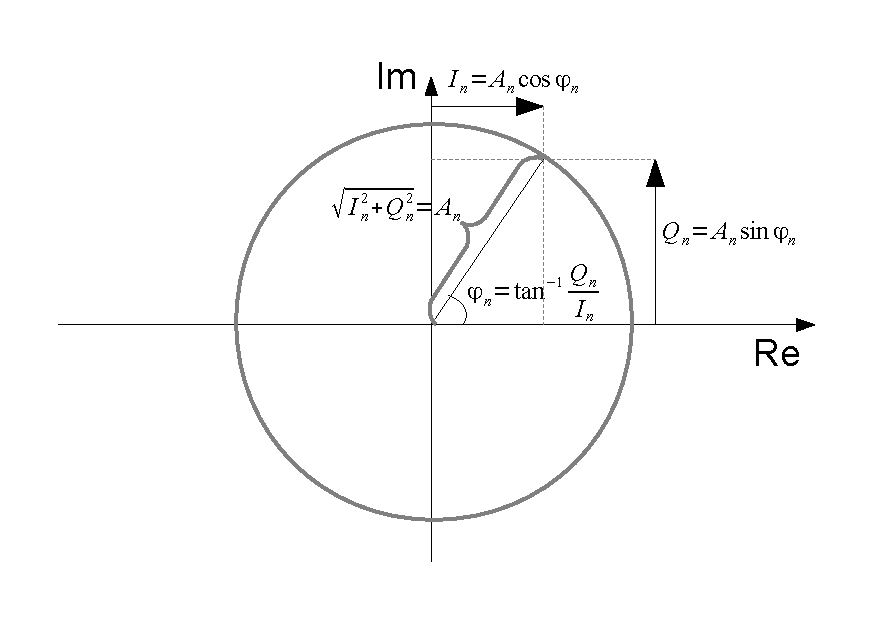
\includegraphics[width=0.9\textwidth]{iqdrawing}
  \caption{Graphical representation of an IQ sample $n$ in the complex plane. All points with the same amplitude $A_{n}$ will lie on the a circle showed in gray. The angle that the sample vector makes with the real axis is the instantaneous phase $\varphi$ of the sample.}
  \label{fig:IQ}
\end{figure}

\chapter{Methodology} 

\section{Analogue Video Signals}

Almost all contemporary video monitors are raster based. The image is transferred from the video controller to the display in scanlines that occur at a specific rate. Each of these scanlines contains a number of pixels which are continuously encoded as a time varying signal. This signal is generated internally in the video controller by an oscillator which runs at the pixel clock rate. The analogue signal is thereafter multiplied by the pixel intensities at the specific time.

Let's assume that the signal started transmitting at time $t=0$, and each video frame contains $y_\text{t}$ scanlines, each of which contains $x_\text{t}$ pixels. The frequency with which frames are being generated is $f_\text{v}$ frames per second. The duration of transmission of each individual pixel is \begin{equation}
\label{eq:tdelta_definition}
t_\text{p}=\frac{1}{x_\text{t} \cdot y_\text{t} \cdot f_\text{v}}
\end{equation}
Note that at time $t$, frame number $n(t)$ started transmission where 
\begin{equation}
n(t)=\lfloor t f_\text{v} \rfloor
\end{equation}
We can assume that the top left corner of a frame has coordinates $(0, 0)$, a pixel at position $(x, y)$ in frame $n(t)$ will start to be transmitted at time
\begin{equation}
T_{(x,y)}= (n(t) x_\text{t} h + y x_\text{t} + x) t_\text{p}
\end{equation}
and will finish transmission before time 
\begin{equation}
T_{(x+1,y)} = T_{(x,y)} + t_\text{p} =(n(t) x_\text{t} h + y x_\text{t} + x + 1) t_\text{p}
\end{equation}
at which the next pixel will start transmitting.

In practice $x_\text{t}$ and $y_\text{t}$ are determined by the screen resolution and $f_\text{v}$ is simply the screen refresh rate. For a typical screen resolution of $width \times height$, it is true that $x_\text{t} \geq width$ and $y_\text{t} \geq height$. The reason is that video signals tend to have additional blanking intervals. This means more pixels are transmitted than what is in the active video region. This gives opportunity for the receiving monitor to synchronise its internal clock, calibrate its colour levels or in case of CRT, allow enough time for the electron beam to return to the beginning of the next line on the screen. The synchronisation timings for personal computers have been standardised by Video Electronics Standards Association (VESA) \cite{vesa}.

In order to decode an individual pixel, the receiving monitor has its own internal oscillator. It locks it to the pixel rate of the incoming signal either via an external clock source or using the blanking intervals. Once it receives the signal for an individual pixel, its amplitude (or binary content in case of digital signal) will correspond to the intensity. This allows the monitor to display the video in real time. If multiple colours are desired, they can be transmitted separately on different wires in the same fashion.

\section{Generated Radio Wave}

\subsection{Signal Equation}
Let's assume the discrete pixels in a video signal have intensities $v_{i} (i \in \mathbb{Z})$ and are being transmitted for a duration of $t_\text{p}=\frac{1}{x_\text{t} \cdot y_\text{t} \cdot f_\text{v}}$ from (\ref{eq:tdelta_definition}). Let's also assume that the shape of the pixel is $p(t)$ where $p(t)=0$ for $|t| \gg \frac{t_\text{p}}{2}$. We know that pixel $i$ starts transmitting at time $t(i)=i t_\text{p}$ (if we assume that that pixel 0 was transmitted at $t=0$). Also the amplitude of the signal of the transmitted pixel is linearly dependant on its intensity $v_{i}$. Then the resulting actual transmitted radio wave in the time domain will have the form 
\begin{equation}
\label{eq:video_signal}
\tilde{v}(t) = \sum\limits_{i=-\infty}^{\infty} v_{i} p(t-i t_\text{p})
\end{equation}
which is a continuous function. (\ref{eq:video_signal}) can be rewritten as a convolution with a Dirac delta function
\begin{equation}
\label{eq:vasconv}
\tilde{v}(t) = p(t) \ast \left( \sum\limits_{i=-\infty}^{\infty} v_{i} \cdot \delta(t-i t_\text{p}) \right) = p(t) \ast \hat{v}(t)
\end{equation}
where
\begin{equation}
\label{eq:vhattdef}
\hat{v}(t) = \sum\limits_{i=-\infty}^{\infty} v_{i} \cdot \delta(t-i t_\text{p}) \text{.}
\end{equation}
Note that this results in infinitesimally short (in time) spikes at values exact integer multiples of $t_\text{p}$ with amplitudes weighted to the pixel intensities at that time. We can view (\ref{eq:vasconv}) as the pixel shape being repeated at intervals of $t_\text{p}$ modulated by $v_{i}$. 

\subsection{Sampling}
We can notice that (\ref{eq:vhattdef}) looks like the result of a continuous signal being sampled at discrete points in time $t_\text{p}$ apart. If we call this hypothetical continuous signal $v(t)$, then we can rewrite the equation so that it reads
\begin{equation}
\hat{v}(t) = \sum\limits_{i=-\infty}^{\infty} v(t) \cdot \delta(t-i t_\text{p}) = v(t) \sum\limits_{i=-\infty}^{\infty} \delta(t-i t_\text{p})
\end{equation}
The requirement is that if $v(t)$ is sampled at discrete intervals $i t_\text{p}$, it should be equal to the corresponding pixel values i.e.\  $v(0)=v_{0}$, $v(t_\text{p})=v_{1}$, $v(2 t_\text{p})=v_{2}$, etc. This would mean that we can precisely obtain the samples from the continuous function by applying the series of Dirac delta functions. However, now we would also like to be able to obtain the continuous signal by only having the sampled values $v_{i}$.This means that we need a unique perfect reconstruction i.e.\  to be able to obtain all $v_{i}$ from $v(x)$ and $v(x)$ from all $v_{i}$. Under the assumption that $v(t)$ is band-limited so that $\mathcal{F}\big( v(t) \big)(f) = 0$ for $|f| < \frac{t_\text{p}}{2}$, the condition is satisfied by the Whittaker--Shannon interpolation formula \cite{shannon1949communication}. It gives us the condition for perfect reconstruction for band-limited digitally sampled signals. It states that the continuous signal could be uniquely reconstructed using $\operatorname{sinc}$ interpolation. If we apply it to our $v_{i}$ samples, it yields
\begin{equation}
v(t) = \sum\limits_{k=-\infty}^{\infty} v_{k} \cdot \operatorname{sinc} \Bigg( \pi \left( \frac{t}{t_\text{p}} - k \right) \Bigg)
\end{equation}
We can verify that when $t=i t_\text{p}$, then $\operatorname{sinc}(\pi (i-k) )$ will always yield $0$ except for when $i = k$ in which case it will be $1$. Therefore we have proved that $v(i t_\text{p}) = v_{i}$.

\subsection{Repetitions}
Now let's revise some mathematical identities. According to the convolution theorem \cite{arfkenconvolution}
\begin{equation}
\mathcal{F} \left\{ g \cdot h \right\} = \mathcal{F} \left\{ g \right\} \ast  \mathcal{F} \left\{ h \right\}
\end{equation}
Which reads: the Fourier transform of a multiplication of two functions is equivalent to the Fourier transforms of the individual functions convolved together. And vice versa
\begin{equation}
\mathcal{F} \left\{ g \ast h \right\} = \mathcal{F} \left\{ g \right\} \cdot  \mathcal{F} \left\{ h \right\}
\end{equation}
The convolution of the Fourier transform of two functions is equivalent to the individual Fourier transforms of the two functions multiplied together.
It could be also shown that:
\begin{equation}
\mathcal{F} \left\{ \sum\limits_{n=-\infty}^{\infty}  \delta(t-n k) \right\} = \frac{1}{k} \sum\limits_{n=-\infty}^{\infty}  \delta \left( t-\frac{n}{k} \right)
\end{equation}
using the last three identities, we can write the Fourier transform of (\ref{eq:vasconv}) as
\begin{multline} 
\label{eq:vspectrum}
\mathcal{F} \left\{ p(t) \ast \hat{v}(t) \right\} = \mathcal{F} \left\{ p(t) \ast \left( \sum\limits_{i=-\infty}^{\infty} v(t) \cdot \delta(t-i t_\text{p}) \right) \right\} = \\
\tilde{V}(f) = \frac{1}{t_\text{p}} P(f) \cdot  \left[ V(f) \ast
\sum\limits_{i=-\infty}^{\infty}  \delta \left( t-\frac{i}{t_\text{p}} \right) \right]
\end{multline}
Where $P(f)$ is the Fourier transform of $p(t)$, $\tilde{V}(f)$ is the Fourier transform of $\tilde{v}(t)$ and $V(f)$ is the Fourier transform of $v(t)$. This simply means that the signal spectrum $V(f)$ repeats at regular intervals throughout the radio spectrum with a frequency of $\frac{1}{t_\text{p}} = x_\text{t} \cdot y_\text{t} \cdot f_\text{v}$. The intensities of the emission at the different frequencies is determined by the shape of the pixel $p(t)$.

For example, for a resolution of $800 \times 600 $ @ $ 60$ fps (ignore blanking intervals for simplicity), we would have a frequency of $\frac{1}{t_\text{p}} = 800 \times 600 \times 60 = 28.8$ MHz. This means that we would expect to find such a signal centred at DC, 28.8 MHz, 57.6 MHz, 86.4 MHz, etc.

In order to obtain the full video signal, we need to know what is the minimum rate at which we need to sample the baseband. We saw from (\ref{eq:vspectrum}) that $V(f)$ repeats at the regular intervals. As a consequence from the Whittaker--Shannon interpolation formula that we used to construct $v(t)$, we know that $V(f)$ is band limited so that $V(f) = 0$ for all $|f| \geq \frac{1}{2 t_\text{p}}$. Therefore we need to have a receiver with a sampling rate of at least $\frac{1}{t_\text{p}}$.

\section{Digital Video Signals}

The analysis above was aimed at analogue signals such as the ones transmitted via VGA. However the majority of contemporary laptops and similar devices don't simply modulate the pixel intensities as analogue voltage amplitudes. Instead, they transmit each pixel as digital bits using FPD-Link (Flat Panel Display Link) to transmit LVDS (Low-voltage differential signalling) signal. For each pixel, 7 bits are transmitted over each of the three wires that determine the resulting RGB colour.

Therefore each bit is transmitted for a duration of $t_\text{b}=\frac{1}{x_\text{t} \cdot y_\text{t} \cdot f_\text{v} \cdot n_\text{b}}=\frac{t_\text{p}}{n_\text{b}}$ where $n_\text{b}$ is the number of bits per pixel which in case of FPD-Link is $n_\text{b} = 7$. Which represents a bit stream of values $c_{k} (k \in \mathbb{Z})$. We defined the $k$-th value of being the $(k \mod n_\text{b})$ bit of the binary number that is used to represent the analogue pixel intensity of pixel number $\left\| \frac{k}{n_\text{b}} \right\|$ (remember, the intensity of pixel number $i$ is denoted as $v_{i}$).

Therefore, we can write the resulting analogue signal as:
$$\tilde{v}(t) = \sum\limits_{k=-\infty}^{\infty} c_{k} b(t-k t_\text{b})$$
where $b(t)$ is the shape of the pixel where $b(t)=0$ for $|t| \gg \frac{t_\text{b}}{2}$.

Now assuming $c(t)$ is the continuous version of $c_{k}$ as in the previous section, we can do the same Fourier analysis on this signal, similar to (\ref{eq:vspectrum}) to obtain:
\begin{multline} 
\mathcal{F} \left\{ b(t) \ast \left( \sum\limits_{k=-\infty}^{\infty} c(k) \cdot \delta(t-k t_\text{b}) \right) \right\} = \\
\frac{1}{t_\text{b}} B(f) \cdot  \left[ C(f) \ast \sum\limits_{k=-\infty}^{\infty}  \delta \left( t-\frac{k}{t_\text{b}} \right) \right]
\end{multline}

This means that we will also get repeating signal throughout the spectrum, this time repeating with a frequency of $\frac{1}{t_\text{b}} = x_\text{t} \cdot y_\text{t} \cdot f_\text{v} \cdot n_\text{b}$. This is $n_\text{b}$ higher than the calculated repetition frequency for analogue signals. For example, Markus Kuhn's laptop was running LVDS with $n_\text{b}=7$ at a video mode of $800 \times 600 $ @ $ 75$ with $x_\text{t} = 1056$ px, $x_\text{t} = 628$ lines and $f_\text{v} = 75$ Hz. He reports receiving the strongest emanations at about $350 MHz$ \cite{kuhn2005electromagnetic}. We can see that this agrees with the theoretical predictions since for his case $\frac{1}{t_\text{b}} = 1056 \cdot 628 \cdot 75 \cdot 7 \simeq 348.2$ MHz.

\section{Reception}

\subsection{Theory}
In order to receive a copy of the video signal, we will need to apply a bandpass filter centred at a multiple of the pixel frequency. The width of the bandpass needs to be the same as the band limited video signal we want to eavesdrop. Then we need to generate an internal clock that runs at the pixel rate and use that to obtain the estimated pixel intensities. Luckily these steps are already done in a typical AM (Amplitude Modulation) receiver. Unfortunately the signal bandwidth is much wider than what a typical off-the-shelf AM receiver can handle.

However some software-defined radio receivers can provide the required bandwidth. The Ettus Research USRP B200 can provide more than 50 MHz of realtime bandwidth which covers what is required to eavesdrop most video signals. Software-defined radios provide the radio samples as a quadrature vector which angle relates to the instantaneous phase in relation to the internal hardware oscillator of the hardware. The size of the vector is proportional to the received amplitude for each sample (refer to Section \ref{sec:IQSampling} for more information). For AM reception, we do not need the phase information since the video signal is being transmitted with a constant frequency. Therefore we can make a simple AM demodulator by taking the length of the vector of each sample. When our digital sampling rate matches the pixel rate, each sample will contain an estimate that relates to the average pixel intensity between time $t(i)$ and $t(i+1)$. For digital signals, it would be related to the bit pattern of the binary value (although this relation may not be unique) that represents the intensity for the current pixel.

\subsection{Practice}
The VESA standard specifies an allowed frequency tolerance for $f_\text{v}$ of 0.5\%. Therefore due to hardware limitations, we might not be able to accurately tune the receiver sampling rate with enough accuracy to match the transmitted pixel rate. This means that some resampling needs to be done in software in order to create a new digital signal that matches as close as possible the transmitted pixel rate in which each sample corresponds to a pixel.

It is also true that we might be able to recover a lot of information from a signal even if our receiver is not capable of sampling the full width of the video spectrum. This means we will only receive a of $v(f)$ with a bandpass filter applied to it. In this case the digital resampling could interpolate the received samples to fit into multiple pixels. Therefore it is useful to introduce a measurement $\kappa$ of how accurate we can reconstruct pixels of $v(t)$. This measurement can be the number of input samples that have gone into constructing a single output pixels. Therefore
\begin{equation}
\label{eq:kappa}
\kappa = f_\text{s} \cdot t_\text{p} = \frac{f_\text{s}}{x_\text{t} \cdot y_\text{t} \cdot f_\text{v}}
\end{equation}
Where as before, $f_\text{s}$ is the receiver sampling rate. If $\kappa \geq 1$, then we can deconstruct individual pixels. If $\kappa < 1$ we are looking at a band-passed version of the signal and consecutive reconstructed pixels will have some interdependencies. Please refer to Figure \ref{fig:samplerates} for a visual comparison of different values of $\kappa$.

\begin{figure}[p!]
\centering
\begin{subfigure}[b]{0.45\textwidth}
  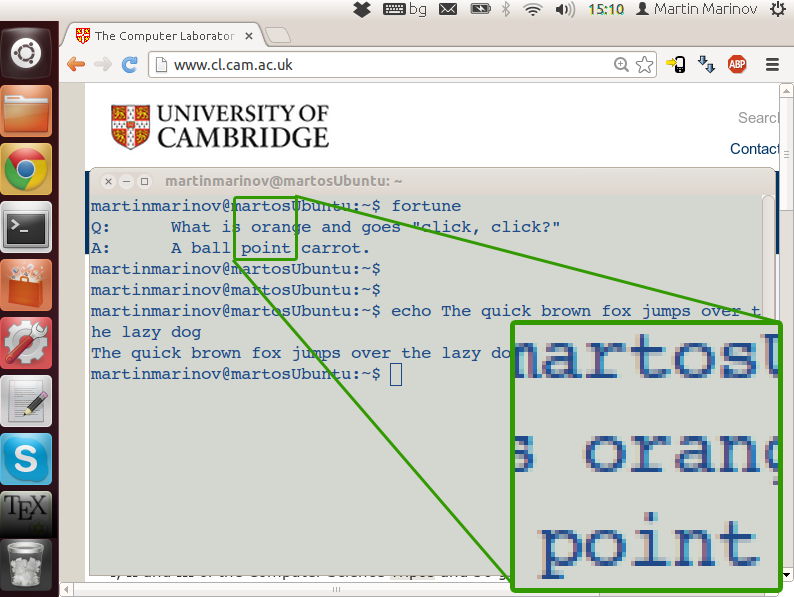
\includegraphics[width=\textwidth]{sr_original}
  \caption{Transmitted image}
\end{subfigure} ~
\begin{subfigure}[b]{0.45\textwidth}
  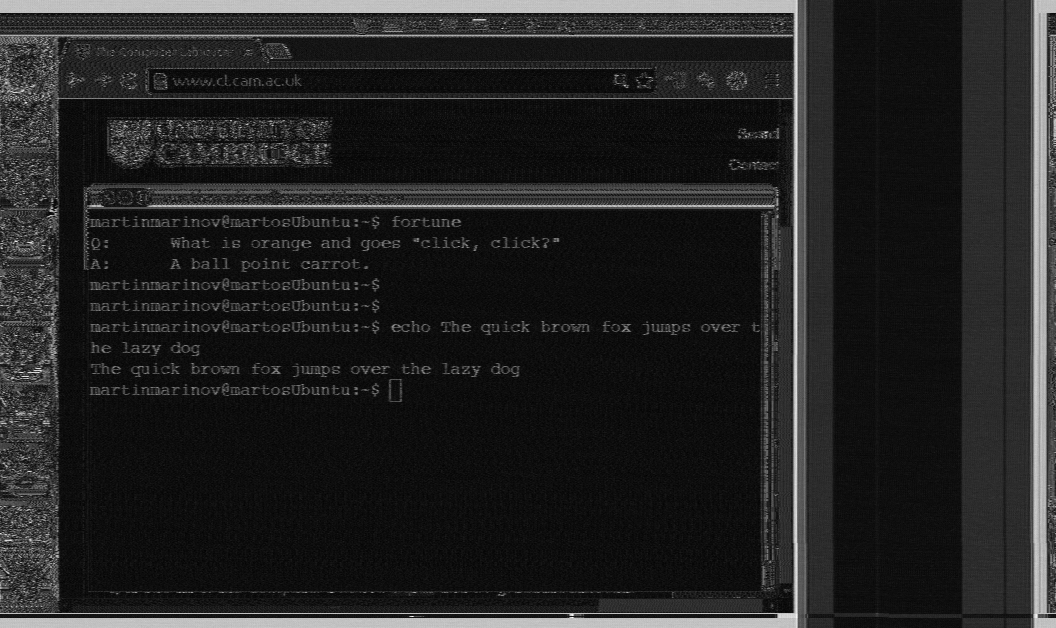
\includegraphics[width=\textwidth]{sr_40MHz_at_190MHz}
  \caption{$\kappa = 1.003$}
\end{subfigure} ~
\begin{subfigure}[b]{0.45\textwidth}
  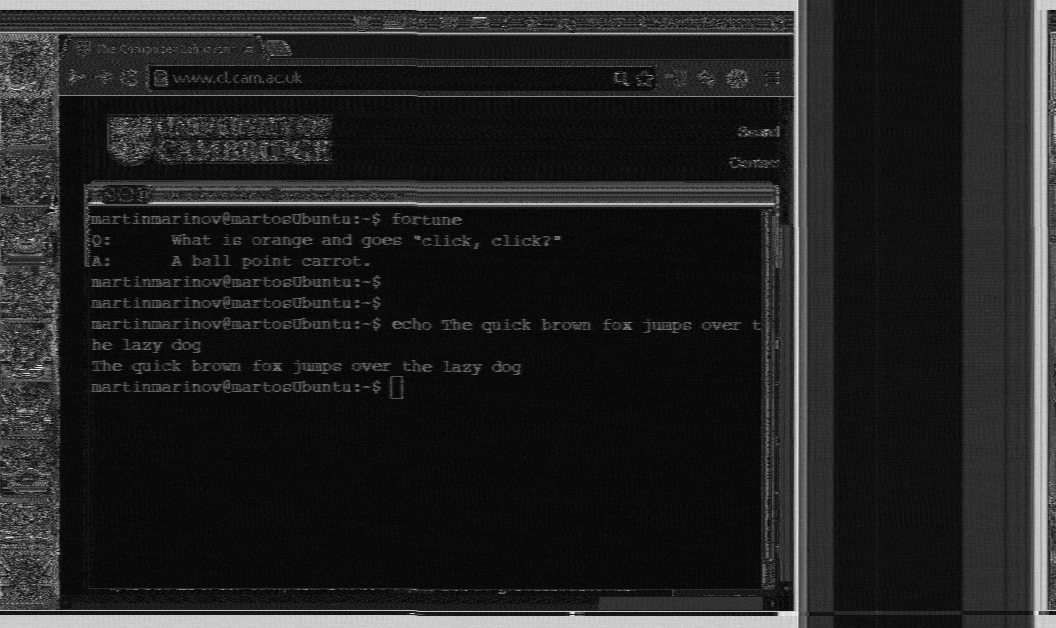
\includegraphics[width=\textwidth]{sr_30MHz_at_190MHz}
  \caption{$\kappa = 0.753$}
\end{subfigure} ~
\begin{subfigure}[b]{0.45\textwidth}
  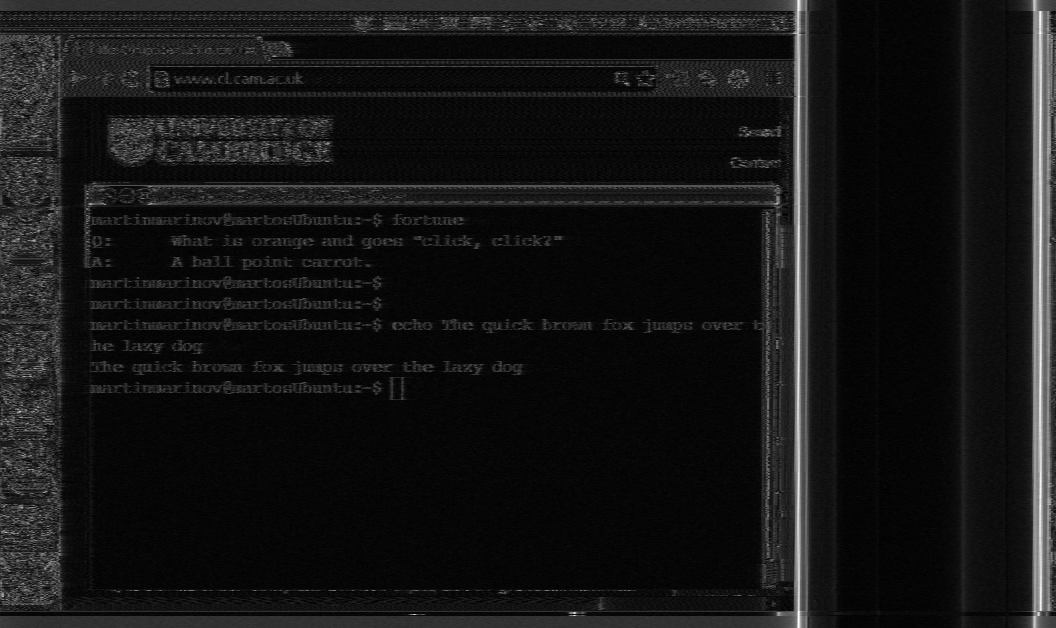
\includegraphics[width=\textwidth]{sr_20MHz_at_190MHz}
  \caption{$\kappa = 0.502$}
\end{subfigure} ~
\begin{subfigure}[b]{0.45\textwidth}
  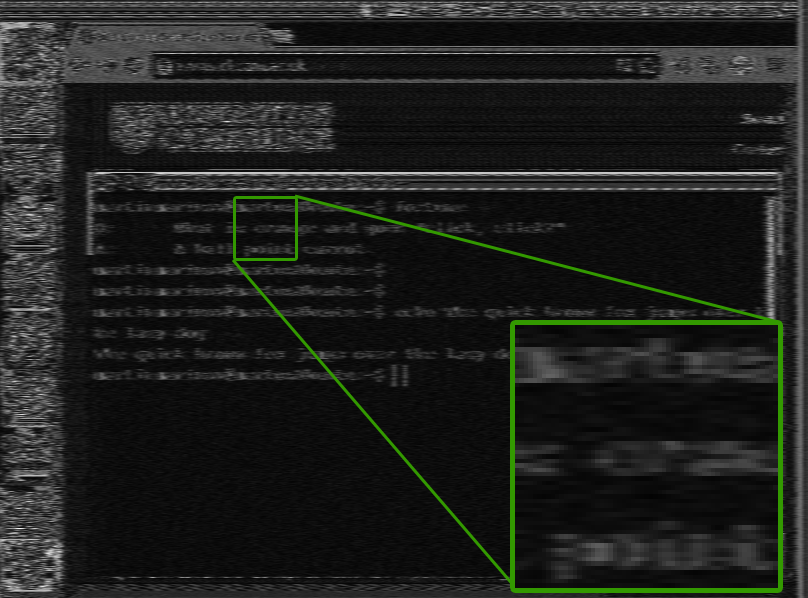
\includegraphics[width=\textwidth]{sr_10MHz_at_190MHz}
  \caption{$\kappa = 0.251$}
\end{subfigure} ~
\begin{subfigure}[b]{0.45\textwidth}
  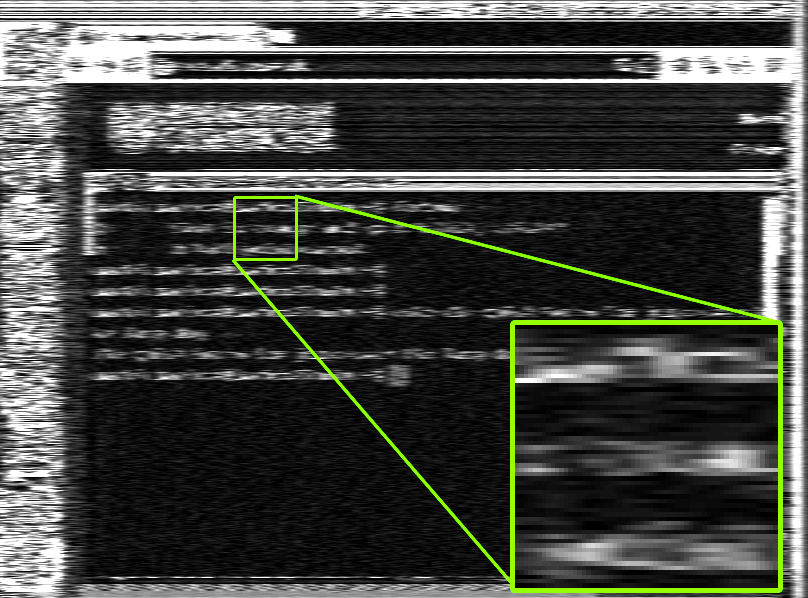
\includegraphics[width=\textwidth]{sr_5MHz_at_190MHz}
  \caption{$\kappa = 0.125$}
\end{subfigure}
\caption{The transmitted image (a) is being sent at a pixel rate of 800x600 at 60 fps with $x_\text{t} = 1056$, $y_\text{t} = 628$ and $f_\text{v} = 60.11$. Each of the screenshots shows the reconstructed image with the receiver (USRP B200) running at different sample rates: (b) 40 MHz, (c) 30 MHz, (d) 20 MHz, (e) 10 MHz and (f) 5 MHz}
\label{fig:samplerates}
\end{figure}

Another possible source of distortions is the usage of multiple wires to transmit colour information. These signals interfere with each other and the resulting pixel intensity becomes a complicated mix of the signals generated in these wires. Therefore colour information would be very difficult to obtain. Nevertheless the outlined strategy allows an eavesdropper to detect changes in colour since this would result in different signal amplitudes arriving at the receiver for each pixel.

\section{Resolution and Framerate Detection}

The outlined method for decoding the video stream relies on us having the exact values for $x_\text{t}$, $y_\text{t}$ and $f_\text{v}$. This is not very practical for a real world attack. We would require the adversary not to have any knowledge of the target system whatsoever. Therefore we would need to infer all of these parameters remotely by exploiting some typical characteristics of a video signal. Namely the fact that the signal is periodic.

As we have already seen, a video signal consists of video frames with width $x_\text{t}$ and height $y_\text{t}$. The speed at which such frames are transmitted is $f_\text{v}$. However most of the time any two consecutive frames would be identical. This would be the case if the victim is looking at static text on the screen. Therefore we can regard the transmitted signal as a repeating periodic signal of a single frame. Which means if we analyse the signal for repeating patterns we should be able to spot the repeating video frames in it and use that to estimate $f_\text{v}$.

\subsection{Introduction to Autocorrelation}
A good way of doing so would be calculating the discrete autocorrelation \cite{bracewell1965autocorrelation} of the incoming signal which is defined as 
$$ R_{vv}(j)=\sum\limits_{i} v_{i} \bar{v}_{i-j} $$
Where $\bar{v}$ is the complex conjugate of $v$ and $j$ is the \textbf{samples lag}. In our case $v$ is the set of real samples, therefore $\bar{v} = v$. Basically the autocorrelation is a measure of the similarity of a signal with itself shifted by a lag. The higher the value of $R_{vv}(j)$ is, the more similar the function is at that lag. Therefore by analysing $R_{vv}(j)$, we would be able to spot any repeating patterns inside $v_{i}$.

Figure \ref{fig:autocorr} shows the discrete autocorrelation of a video signal that was captured using the Mirics USB dongle at 8 MHz (i.e.\  $8,000,000$ samples per second) sampling rate. The vertical axis is logarithmic, containing the decibels of the autocorrelation i.e.\  $10 \log_{10}( R_{vv} )$. The horizontal axis contains the time lag in milliseconds. This was converted from the lag in samples $j$ by $x = \frac{j}{f_\text{s}}$.

\begin{figure}[h]
\centering
  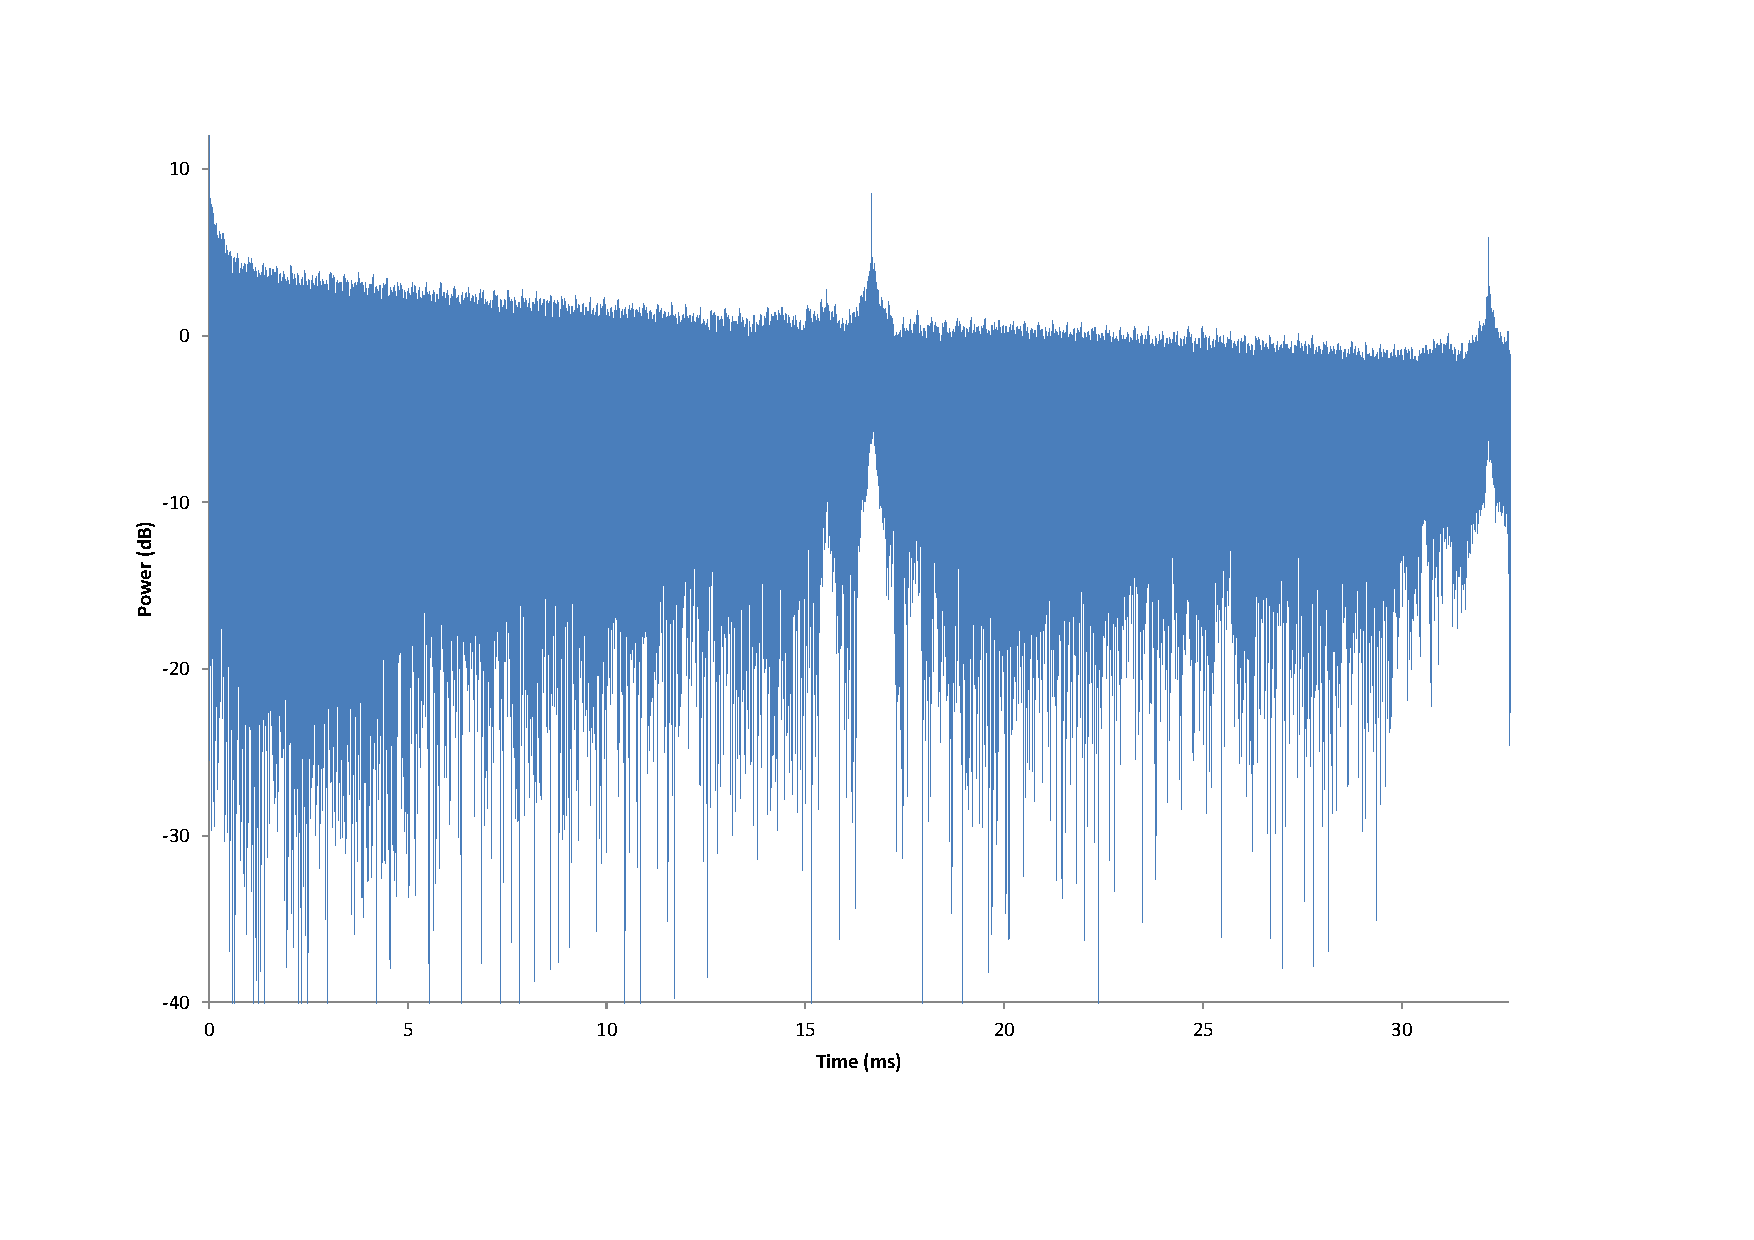
\includegraphics[width=0.96\textwidth]{autocorr}
  \caption{Autocorrelation of a signal}
  \label{fig:autocorr}
\end{figure}

This particular example consists of $524,288$ samples which is $65.536$ milliseconds of recording. This allows us to estimate the autocorrelation up to half of it, namely $32.768$ milliseconds. The reason is because $R_{vv}(j)=-R_{vv}(j)$ due to symmetry. We can see a peak at $16.672$ milliseconds which corresponds to a frequency of $f_\text{v} = \frac{1}{0.016672} = 59.98$ Hz. This is our estimate for $f_\text{v}$. And it makes sense, $60$ Hz is a common refresh rate for contemporary video displays.

\subsection{Aliasing}
We should be able to see the peak repeating again at $2 \times 16.672 = 33.344$ ms. This is analogous to comparing every two consecutive frames with every two other frames. However, as this falls just outside our window it would be seen as an alias at $65.536-33.344 = 32.192$ ms. The same applies for the third peak at $3 \times 16.672 = 50.016$ ms which would be comparing each block of three consecutive frames with the next three. This will alias at $65.536 - 50.016 = 15.52$ ms. This explains the second small peak we see on the left of the main one at $16.672$ ms but we see that the difference in its power is already several decibels lower. Therefore any further aliasing induced would be even smaller.

It is therefore important to choose the number of samples to be used for the autocorrelation wisely in order to avoid aliasing. We need to have enough full frames in our data so that the autocorrelation can physically work. The minimum frequency we can get from an autocorrelation is $\frac{2 s}{N}$ where $N$ is the total number of samples that we are doing the autocorrelation on. It could be easily shown that the second alias is
\begin{equation}
\hat{f}_{2}(f) = \frac{1}{\frac{2}{f_\text{min}}-\frac{2}{f}} = \frac{1}{\frac{N}{f_\text{s}}-\frac{2}{f}}
\end{equation}
Where $f$ is the frequency we are going to see the alias for. Therefore if we want to be able to pick up a repeating pattern of at least $f_\text{min} = 50$ Hz, we would need $\frac{2 s}{50}$ which in our case is $320,000$ samples. However having such a small number of samples if we observe a signal at 85 Hz we would discover a strong alias at $\frac{1}{\frac{320,000}{8,000,000}-\frac{2}{85} } = 60.714$ Hz which would be very misleading and will look like a legitimate signal at $60.714$ Hz. 

Let us assume $f_\text{low} \leq f_\text{v} \leq f_\text{hi}$. In order to minimise aliasing, we can try to keep the second alias $\hat{f}_{2}(f_\text{src})$ outside this range. Therefore we need to pick the number of samples so that
$$f_\text{low} \geq \hat{f}_{2}(f_\text{low}) \equiv \frac{1}{\frac{N}{f_\text{s}}-\frac{2}{f_\text{low}}}  \,\,\,\,\ \text{or} \,\,\,\,\ f_\text{hi} \leq \hat{f}_{2}(f_\text{hi}) \equiv \frac{1}{\frac{N}{f_\text{s}}-\frac{2}{f_\text{hi}}}  $$
Which means that
$$ N \geq 3 \frac{f_\text{s}}{f_\text{low}} \,\,\,\,\ \text{or} \,\,\,\,\ N \leq 3 \frac{f_\text{s}}{f_\text{hi}} $$
and don't forget that in the same time we have the condition
$$N \geq 2 \frac{f_\text{s}}{f_\text{low}}$$
so in the end, in order to eliminate the second alias in the desired region from $f_\text{low}$ to $f_\text{hi}$ in the autocorrelation, we would need to choose the number of samples to be
\begin{equation}
\label{eq:autocorraliasingcondition}
N \geq 3 \frac{f_\text{s}}{f_\text{low}}
\end{equation}
To paraphrase this result, we will need to do the autocorrelation on at least 3 frames worth of samples for the lowest frequency in our range $f_\text{low}$ to avoid second order aliasing interfering with our plot.

\subsection{Number of Lines in a Frame}

We were able to estimate $f_\text{v}$ using an autocorrelation and eliminate aliased signals in the frequency window that we are looking to detect repetitions. However, we still have not estimated neither $x_\text{t}$, nor $y_\text{t}$. As a matter of fact we might not be able to measure $x_\text{t}$ at all. The reason is that $x_\text{t}$ might be a continuous signal and could potentially contain any number of pixels. However, each line of $x_\text{t}$ pixels repeat $y_\text{t}$ times in a frame which includes the blanking intervals. Therefore we can use their repeating nature of the blanking intervals to estimate $y_\text{t}$ from the autocorrelation plot.

For this reason we need to zoom in to our plot. Refer to Figure \ref{fig:autocorr_zoomed} which is a zoomed out version of the figure we saw in the previous subsection. If we still have our allowed $f_\text{v}$ window between $f_\text{low}$ and $f_\text{hi}$, then we can assume that $y_\text{t}$ also spans between $h_\text{low}$ and $h_\text{hi}$. We would therefore expect to see a peak between $\frac{1}{f_\text{hi} \cdot h_\text{hi}}$ and $\frac{1}{f_\text{low} \cdot h_\text{low}}$ milliseconds. If we detect a peak at time $t_\text{peak}$, then this would correspond to $y_\text{t} = \left\| \frac{1}{t_\text{peak} \cdot f_\text{v}} \right\|$ where $\|$ represents rounding to the nearest integer. Note that we should have already estimated $f_\text{v}$.

\begin{figure}[h]
\centering
  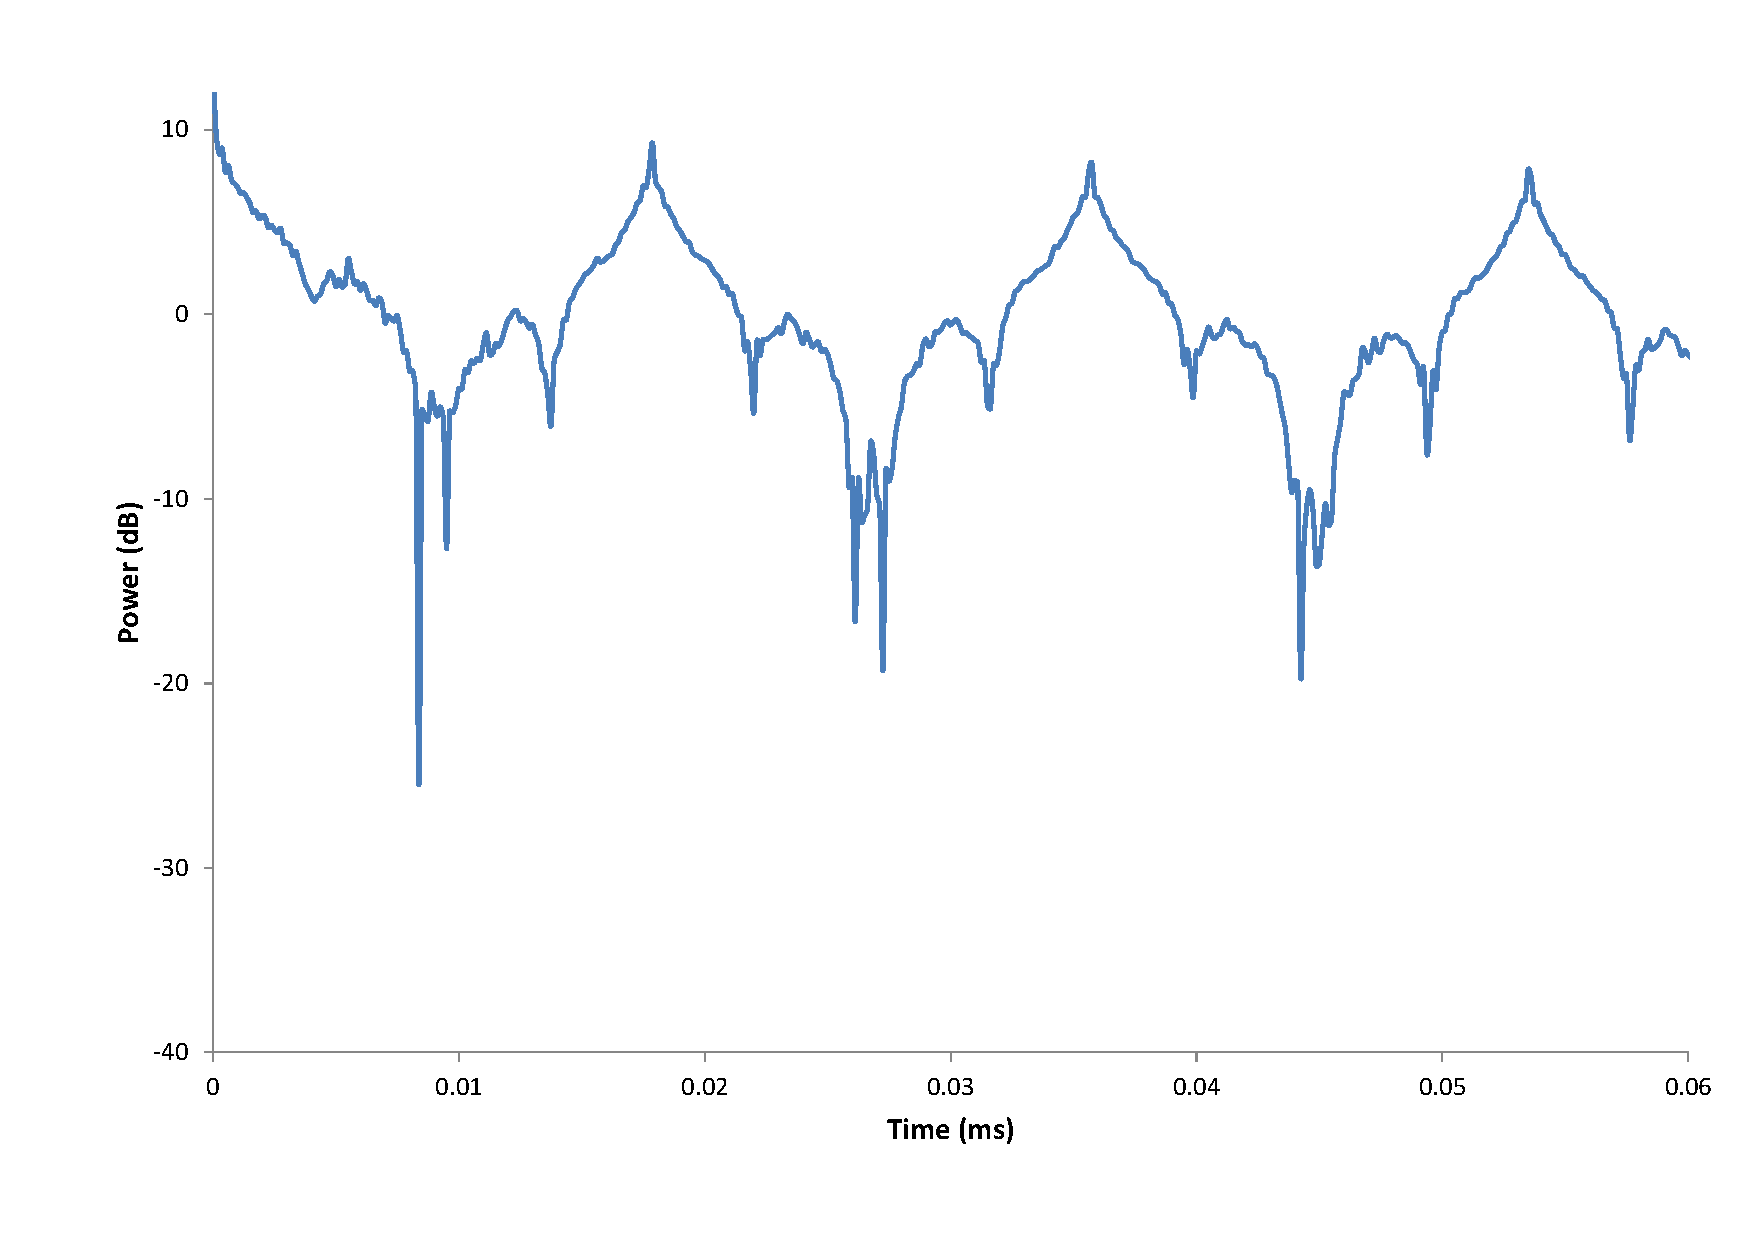
\includegraphics[width=0.96\textwidth]{autocorr_zoomed}
  \caption{Zoomed in version of \ref{fig:autocorr}}
  \label{fig:autocorr_zoomed}
\end{figure}

Our plot shows a peak at $0.017875$ milliseconds. Since we already estimated $f_\text{v} = 59.98$ Hz, then $y_\text{t} = \left\| \frac{1000}{0.017875 \times 59.98} \right\| = 933$ lines. If we look at a list of VESA video modes, we can see that there is a conveniently close video mode that corresponds to $y_\text{t} = 933$ and $f_\text{v} = 59.98$. It is the $1440 \times 900$ @ $60$ video mode with $x_\text{t} = 1904$ pixels, $y_\text{t} = 932$ lines and $f_\text{v}=60$ Hz. Therefore we could use the value of $x_\text{t} = 1904$ for our estimate of the number of pixels in a row. This will keep the aspect ratio correct.

We should not worry about aliasing since the number of samples in the autocorrelation is much bigger than our range. We can see on the plot the autocorrelation values repeating for each two lines, each three lines, etc. This results in a number of peaks repeating with the rate at which individual lines repeat in the video signal.

\subsection{Errors}

There is a limit on how accurately one can determine $f_\text{v}$ and $y_\text{t}$ using the outlined autocorrelation method. This depends on the sampling rate of the device. The resolution of the autocorrelation is $\delta f = \frac{1}{f_\text{s}}$. Therefore we can only say that if there is a peak at $t_{x}$ in the autocorrelation, then we have a repeating component in the signal with a frequency $f_{x} \pm \delta f$.

The accuracy at which we can determine $y_\text{t}$ depends both on the accuracy of $f_\text{v}$ and $t_\text{peak}$ and can vary. Furthermore $y_\text{t}$ should be rounded to an integer (we can only display an integer number of lines on a PC screen) which introduces further errors. Our definition for $y_\text{t}$ is
$$y_\text{t} = \left\| \frac{1}{t_\text{peak} \cdot f_\text{v}} \right\| \pm (\delta y_\text{t} + 0.5)$$
Where $0.5$ comes from the rounding. Also the uncertainties in $t_\text{peak}$ and $f_\text{v}$ are $\delta f$ since both are being read from the same autocorrelation plot in milliseconds. In order to do error propagation, we need to take the partial derivatives with respect to $f_\text{v}$ and $t_\text{peak}$.
$$\frac{\partial h}{\partial f_\text{v}} = - \frac{1}{t_\text{peak} \cdot f_\text{v}^2}
 \,\,\,\,\ \text{and} \,\,\,\,\ \
\frac{\partial h}{\partial t_\text{peak}} = - \frac{1}{f_\text{v} \cdot t_\text{peak}^2}$$
So for the uncertainty in $y_\text{t}$, we have
$$\delta y_\text{t} =
\sqrt{\left( \frac{\partial h}{\partial f_\text{v}} \delta f_\text{v} \right)^2 + \left( \frac{\partial h}{\partial t_\text{peak}} \delta t_\text{peak} \right)^2} = 
\sqrt{\frac{1}{f_\text{v}^2} + \frac{1}{t_\text{peak}^2}} \times \frac{\delta f}{f_\text{v} \cdot t_\text{peak}}$$
We can also observe that the larger the sample rate gets, the smaller $\delta f$ and $\delta t$ get.

\chapter{Practical attack} 

Before explaining how the software works internally, let's present a demonstration of a practical video eavesdropping attack. Its main aim is to show the ease with which such an attack could happen. In the meantime this will give an opportunity to explain the characteristics of the received signal and how they are exploited.

As in the real world, we will start with no knowledge of the victim's system. We will estimate the frequency at which the emission strength has the best Signal to Noise Ratio (SNR). We will then analyse the signal to detect the resolution and refresh rate of the screen. We will afterwards lock onto the signal and try to recover the original video. We will also discuss some techniques that could be utilized to improve the quality of the image.

\section{The Setup}

The choice for a Sfront-end for this demonstration is a USRP B200\footnote{Refer to \ref{sec:hw} Hardware for discussion on currently available Sdevices.}. Depending on the particular requirements, an attacker might prefer mobility over accuracy and choose the smaller Mirics FlexiTV\texttrademark MSi3101 SUSB Dongle. However, for this demonstration we will attempt to obtain the highest possible resolution. Therefore we need an Sradio that is capable of obtaining a wide bandwidth. This makes the 32 MHz of Bandwidth that the USRP provides a much better choice than the 8 MHz available from the Mirics dongle.

[Antenna]

[Location of victim]

[Victim's fonts]

\section{Preparation}

\chapter{Implementation} 

\section{Hardware}
\label{sec:hw} 

\begin{figure}[h!]
 
  \centering
    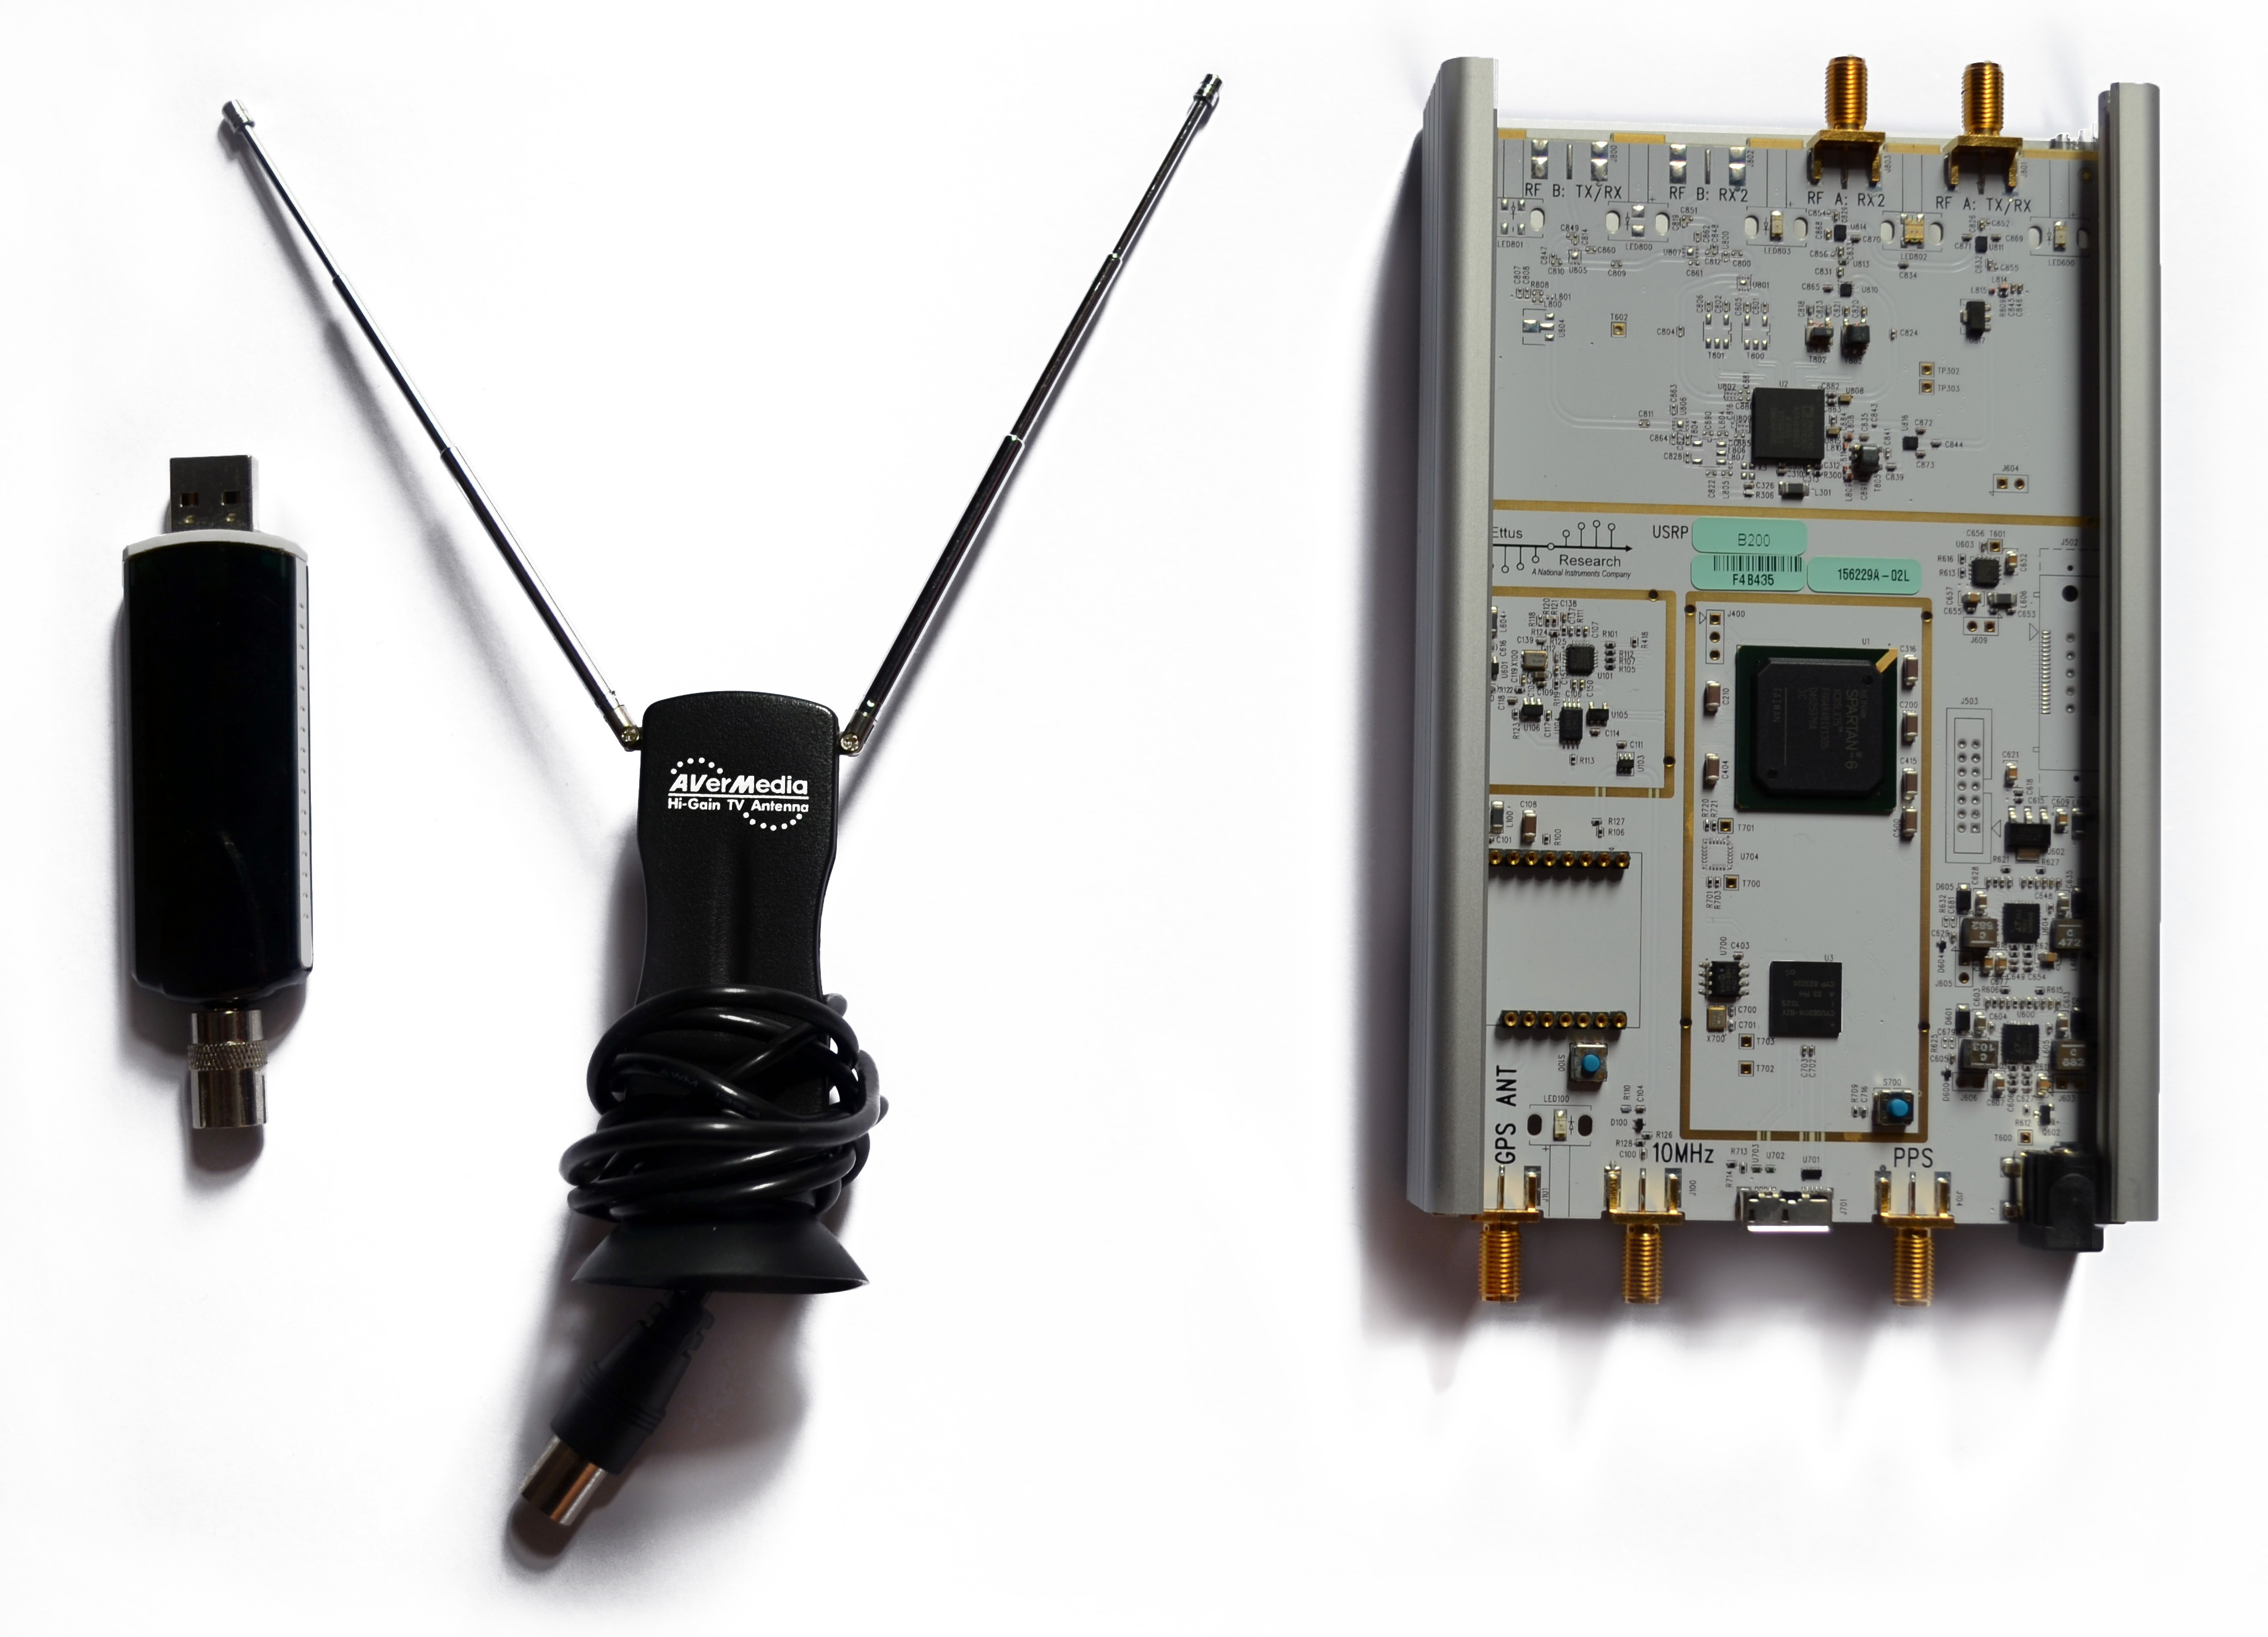
\includegraphics[width=0.9\textwidth]{equipment}
    \caption{From left to right: MSi3101, AverMedia antenna and USRP B200}
\end{figure}

There is a wide range of off-the-shelf Shardware front-ends that could be used with the system. An attacker can choose one depending on their requirements. A quick overview of some of the supported available hardware is outlined below.

\subsection{Ettus Research USRP}

\begin{tabular}{ll}
	Maximum sampling rate: & 56 Mhz (B200) \\
	Frequency Range: & 70 MHz - 6 GHz \\
	Dimensions: & 97 mm $\times$ 155 mm $\times$ 15 mm (B200) \\
	OS support: & All platforms (Windows support via ExtIO) \\
	Dropped samples detection: & Yes (Except on Windows)
\end{tabular}

The maximum sampling rate varies between the different models as well as the dimensions. I have used the USRP B200 throughout this report.

Pros:
\begin{itemize}
	\item A variety of models available in multiple price ranges.
	\item High enough sampling rates for most eavesdropping scenarios.
\end{itemize}

Cons:
\begin{itemize}
	\item Some models need external power supply. B200 in particular does not.
	\item May need some analogue preconditioning for good eavesdropping results.
\end{itemize}

\subsection{Mirics FlexiTV\texttrademark MSi3101}

\begin{tabular}{ll}
	Maximum sampling rate: & 8 Mhz \\
	Frequency Range: & 64 MHz - 240 MHz and 470 MHz - 960 MHz \\
	Dimensions: & 25 mm $\times$ 80 mm $\times$ 10 mm \\
	OS support: & Windows only \\
	Dropped samples detection: & Yes
\end{tabular}

It is the best low end solution but it won't achieve the receiving distance or the quality that one would get with a higher end device.

Pros:
\begin{itemize}
	\item Portable and unsuspicious looking -- just a typical USB dongle.
	\item Inexpensive -- under \pounds 100.
\end{itemize}

Cons:
\begin{itemize}
	\item Low sampling rate and low sensitivity. Good eavesdropping results would be obtained if the target screen resolution is low enough so that $\kappa$ (refer to (\ref{eq:kappa}) for definition) is reasonable and the signal is strong enough.
	\item Tuning gap between 240 MHz and 470 Mhz. If the emanations fall within this range, the Mirics dongle will fail to pick them up.
\end{itemize}

\subsection{Windows ExtIO}

The plug-in supports variety of devices. It is a standard plug-in that is used in a number of software defined radio solutions. However, it does not take into account for dropped samples. This means that if sample loss did occur, this would be very visible on the screen rendering eavesdropping practically difficult. It also only runs on Windows.

\subsection{Antennas and Preconditioning}

For the experiments in this report, I have used a small dual-pole antenna by AverMedia designed for digital TV reception. This showed to be enough for eavesdropping from an adjacent room to the one containing the target device. However, for impressive demos that could potentially operate from several tens of meters, Kuhn recommends some additional analogue preconditioning.

Kuhn experimented with a tunable band pass filter and a 30 dB antenna amplifier before the B200 to improve the noise level. He comments that the setup delivers comparable quality to the highly specialised Dynamic Sciences R1250 receiver that he used in his experiments \cite{kuhn2003compromising}. He also used a professional log-periodic antenna for improved reception.

\section{Architecture}

The whole system consists of two parts - a library (called \textbf{TSDRLibrary}) and a host program. The library is the main deliverable of the project. It is responsible for decoding the emanated signal -- from obtaining the data from the hardware to processing it. However it can't run as a stand-alone application. It needs a host program to control it via an API (defined in \textit{TSDRLibrary.h}) and to receive the decoded video frames. The host program could be written in any programming language that can use native libraries.

However, the package also comes with a pre-built Java based host program. The provided implementation allows for full manual control over the library via a graphical user interface (GUI). It is very useful for real-time monitoring and interacting asynchronously with the library while the processing is taking place. In practice it is a single executable that has TSDRLibrary built in. This is what the report has been referring to as ``the system'' so far -- the Java GUI combined with TSDRLibrary. An end user would never notice that there is another layer underneath the GUI. All of the examples and screen-shots given here have been obtained via the provided Java based GUI while it is controlling TSDRLibrary.

\subsection{The Library}

The library relies on plugins (called \textbf{TSDRPlugin}) to provide a stream of IQ samples and means to control the Shardware in real time. The data sources are shared libraries that are dynamically loaded at runtime by the TSDRLirbary.

The host program's job is extremely simplified. In a nutshell, it sets up the library and runs it. Every time there is a new video frame available, a callback would be invoked via TSDRLibrary so that the host program could process the frame (display it, save it, etc). An expected sequence of API calls to get video data would be:

\begin{enumerate}
	\item Dynamically load the library (if it is not statically compiled with the host program) using the methods provided by the specific operating system. This will give the host program access to the TSDRLibrary APIs.
	\item Allocate an instance of the processing pipeline with \textit{tsdr\_init}.
	\item Set target display resolution and frame rate with \textit{tsdr\_setresolution}. This could be called interactively while the processing is running to dynamically change the parameters at runtime.
	\item Load a pre-compiled plug-in by invoking \textit{tsdr\_loadplugin} specifying the location of the shared library that represents the plugin and any parameters that the user wants to pass to the plug-in. This plugin will talk to the hardware and provide a steam of IQ data to the library for processing.
	\item Start the processing by running \textit{tsdr\_readasync}. The current thread would be used to start polling the hardware so it will block until processing has finished.
	\item The \textit{tsdr\_init} and \textit{tsdr\_readasync} allow for callback functions to be registered with TSDRLibrary. The callbacks are just C functions that reside in the host program that will be called as soon as a new video frames, autocorrelation data or other messages are available. Processing data within those callbacks is not thread safe.
	\item Call \textit{tsdr\_stop} to stop the processing and unblock the thread that originally called \textit{tsdr\_readasync}. Soon after calling \textit{tsdr\_stop}, the callbacks will stop receiving data.
\end{enumerate}

If the plug-in supports it, \textit{tsdr\_setbasefreq} can be used to set the base frequency of the hardware device. A few other API commands allow the host program to do manual position adjustment of the video frame, control the amount of lowpass applied and set the gain of the hardware device (if supported). There are some advanced features that could be turned on using the \textit{tsdr\_setparameter} API call which include the automatic frame borders detection, automatic frame rate synchronisation and a few other tweaks to the digital signal processing pipeline. It is up to the host program to use the autocorrelation to determine resolution and framerate which gives enough room for flexibility.

Each API call can return an error code in case it fails. The host application can also read a verbose version of the error message using the \textit{tsdr\_getlasterrortext} API call. This allows for intuitive and simple error handling.

\subsection{Data Flow}

\begin{figure}[h]
  \centering
    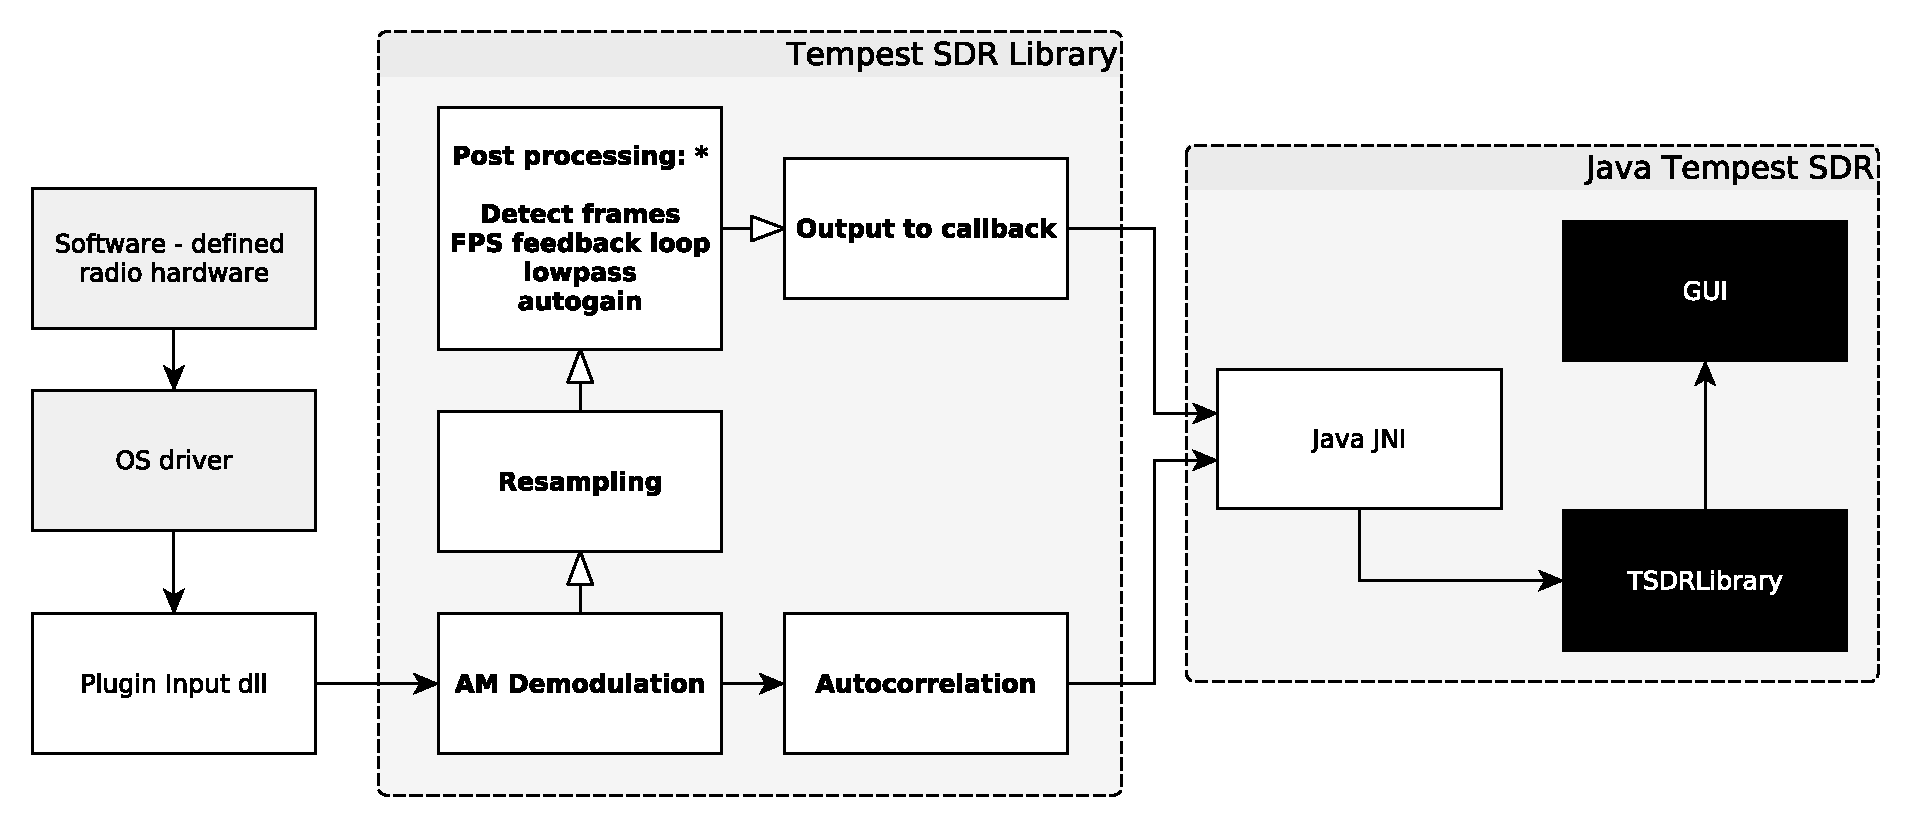
\includegraphics[width=\textwidth]{systemoverview}
    \caption{Data processing in the system using the Java GUI. Bold text represents different native threads. White background means code is written in C. Black background means code is written in Java. Gray background is for operating system related processes and external hardware. Arrows with white ends represent points where data could be dropped due to performance reasons. Arrows with black ends represent transferring full data that was processed in the previous step. The star on the Post processing stage means that the outlined sub-stages could be executed in different order depending on user preferences.}
    \label{fig:architecture}
\end{figure}

Figure \ref{fig:architecture} outlines the data flow and data processing paths within a typical set-up of the system\footnote{If instead the data is read from a file or network, we can regard the ``Software - defined radio hardware'' as the hard drive or the network layer.}. It goes through the following steps:

\begin{enumerate}
	\item RF data is converted into IQ samples in the Sdevice. These samples are sent to the PC for processing.
	\item The hardware driver in the OS receives the samples and possibly queues them.
	\item A TSDRPlugin either continuously polls the driver or receives a callback from it as soon as a block of data is available. It obtains the block of data and sends it to the TSDRLibrary via a callback.
	\item The IQ data is inside TSDRLibrary. AM demodulation is done on the data. This runs in a separate thread so that the TSDRPlugin will have the chance to receive new data from the device as quickly as possible. The demodulated data is provided to the Autocorrelation thread that will calculate the autocorrelation of the incoming signal and notify the host program. If TSDRPlugin reports any dropped samples between calls, the autocorrelation is reset (we only want continuous data accumulated for autocorrelation).
	\item The resampling logic runs in a separate thread. It matches the rate of the data from the sampling rate of the device $f_\text{s}$ to the expected rate of $x_\text{t} \cdot y_\text{t} \cdot f_\text{v}$.
	\item Here some digital signal processing is done in a separate thread to enhance the signal. The order with which the operations are applied depends on the settings that a user will supply. By default the synchronisation pulses of a video frame are detected first. If the user has selected auto tracking, the current position of the horizontal blanking interval is compared with the last one. This gives a rough estimate on whether $f_{fps}$ is off by a couple of parts per million from the real value. The process allows for keeping the picture steady on the screen. Then lowpass in the time domain is done (a.k.a. motion blur) to de-noise a weaker signal using averaging. Finally, an autogain algorithm makes sure that the full dynamic range of the signal is equally utilised for the final image.
	\item Here the host application receives a video frame via a callback. It is up to the host application to determine what to do with it. It can take as much time as it wants since this runs in a separate thread.
	\item The signal leaves the library and goes into the host application. In this example this is our Java GUI. A Java Native Interface (JNI) code marshals the incoming data to a Java friendly format which is then passed to the Java Virtual Machine and the particular class instance that has invoked the whole processing.
	\item Once the data arrives at the TSDRLibrary class instance, the main GUI will receive a notification via a callback and will dispatch the bitmap to be drawn on the screen.
\end{enumerate}

The biggest problem faced was synchronising dropped samples. To illustrate the issue, imagine we are receiving samples at a rate of $50$ mega samples per second. If each sample contains two floating point values (the I and the Q component), each of which being $4$ bytes of data, then the total data rate coming from the hardware would be $8 \times 50 = 400$ megabytes per second! This is a huge amount of data. Since the configuration is running on a non-real-time operating system, the CPU might not be able to cope with such a fast stream. Furthermore there could be some hardware limits enforced as well, for example maximum throughput of the bus that is being used to transmit the data from the Sdevice to the PC.

This means that we will have a lot of dropped samples coming from the device. At the same time, even if we don't have any dropped samples, the CPU can still fail to process all of the desired data in real-time. This means that, in order to have the system run interactively, some samples that can't be processed in real-time should be dropped. This would allow for fresh data to be collected for processing. However having even a couple of dropped samples is a problem. This is because video is continuous. Dropping a few pixels means that the whole frame synchronization could be broken.

Therefore the library employs an algorithm that allows it to drop samples only an integer multiple of $x_\text{t} \times h$ at a time. This means that even if a single sample was dropped before processing, the algorithm will enforce a whole batch of $x_\text{t} \times h$ samples to be dropped instead. This means that when the next frame arrives, it will start processing from where the previous frame had dropped samples. Therefore the picture will look seamless to the end user since the dropped samples will actually result in a lower frame-rate in the host application. This approach allows the system to run even on not so powerful configurations and still produce some output. Such synchronization points are denoted as white arrows on Figure \ref{fig:architecture}.

\section{Digital Signal Processing}

\subsubsection{Demodulation}

\subsubsection{Re-sampling}

\subsubsection{Auto Gain}

\subsubsection{Low-pass}

\subsection{Frame Synchronization}

\subsection{Resolution Detection}

\subsubsection{Frame Synchronization}

\subsection{Experimental: Extended Bandwidth}

\subsection{Main Library}

\subsection{JavaGUI}

\subsubsection{Multiplatform}

\subsubsection{Graphical Interface}

\subsubsection{Visualisation}

%\subsection{Testing and Benchmarking}

\chapter{Summary and Conclusions} 

\subsection{Encountered Issues}

[Summarize results]

[potential future work]

\appendix
\singlespacing

\bibliographystyle{unsrt} 
\bibliography{dissertation} 

\end{document}
